\subsection{List of requirements}
    \begin{center}
        {\renewcommand{\arraystretch}{2}
        \begin{longtable}{L{2cm}L{12cm}}
            \hline
            \textbf{R1} & Visitors are allowed to register as customers through the CLup application \\
            \hline
            \textbf{R2} & The store manager is allowed to register as store manager through the CLup web app \\
            \hline
            \textbf{R3} & Customers are allowed to log in inside the application \\
            \hline
            \textbf{R4} & The store manager and the employee are allowed to login in inside the web application \\
            \hline
            \textbf{R5} & The store manager can insert and edit store information \\
            \hline
            \textbf{R6} & The store manager can create and edit the employees' accounts associated to his/her store \\
            \hline
            \textbf{R7} & The employee can line up a visitor who asked for that and can give him/her the number associated with the position in the queue \\
            \hline
            \textbf{R8} & The employee can report the entrance related to a line up number or a visit and the exit of each person from the store \\
            \hline
            \textbf{R9} & The line up numbers and the visits are invalidated after a period of time if not used to enter the store \\
            \hline
            \textbf{R10} & The employee can see the line up numbers/visits that are allowed to enter the store \\
            \hline
            \textbf{R11} & The CLup system notifies the employee when it's time to call a visitor who previously asked to line up at the entry point \\
            \hline
            \textbf{R12} & The store manager can see charts and analysis related to entrances made with the QR code \\
            \hline
            \textbf{R13} & Customer can generate a QR code to enter the store \\
            \hline
            \textbf{R14} & The CLup system can acquire the scanned QR code \\
            \hline
            \textbf{R15} & The CLup application has a section to line up \\
            \hline
            \textbf{R16} & The CLup application shows the estimated queue waiting time, the queue size, the estimated travel time and the number related to the position in the queue \\
            \hline
            \textbf{R17} & The application monitors the customer's position and computes the estimated travel time \\
            \hline
            \textbf{R18} & The application notifies the customer when the estimated queue waiting time is near the estimated travel time \\
            \hline
            \textbf{R19} & The system generates a unique (in an appropriate time interval) number to identify the position in the queue \\
            \hline
            \textbf{R20} & The system pushes forward the queue based on the reported exits and the scheduled visits \\
            \hline
            \textbf{R21} & The CLup application has a section to book a visit \\
            \hline
            \textbf{R22} & The CLup application shows available time slots for visits \\
            \hline
            \textbf{R23} & The system schedules visits based on related details \\
            \hline
            \textbf{R24} & The customer can insert additional details like what he/she is going to buy, the estimated visit duration or what departments he/she will go to) \\
            \hline
            \textbf{R25} & The CLup system can compute the estimated visit duration for long term customers based on previous visits \\
            \hline
        \end{longtable}}
    \end{center}

\subsection{Mapping}
    \begin{center}
        {\renewcommand{\arraystretch}{2}
        \begin{longtable}{L{2cm}L{6cm}L{6cm}}
            \hline
            \textbf{Goal} & \textbf{Requirements} & \textbf{Domain assumptions} \\
            \hline
            \textbf{G1} & R1, R2, R3, R4, R6 & D5, D18, D19 \\
            \hline
            \textbf{G2} & R3, R4, R6, R8, R9, R11, R17, R18, R19, R20 & D1, D3, D4, D5, D7, D8, D10, D14, D15, D18, D19 \\
            \hline
            \textbf{G3} & R3, R4, R6, R8, R10, R14 & D3, D7, D11, D12, D13, D16, D18, D19 \\
            \hline
            \textbf{G4} & R4, R6, R7 & D2, D3, D6, D12, D13 \\
            \hline
            \textbf{G5} & R4, R5, R6, R7, R8, R10, R15, R20, R21, R23 & D1, D2, D5, D6, D7, D15, D17, D18, D19 \\
            \hline
            \textbf{G6} & R4, R6, R7, R9, R11 & D1, D2, D3, D5, D6, D8, D10, D15, D18, D19 \\
            \hline
            \textbf{G7} & R3, R21, R22, R24 & D1, D3, D5, D9, D10, D13, 18 \\
            \hline
            \textbf{G8} & R3, R13, R15, R16, R19 & D1, D2, D3, D5, D9, D10, D13, D18 \\
            \hline
            \textbf{G9} & R4, R5, R12, R14 & D1, D5, D11, D18, D19 \\
            \hline
            \textbf{G10} & R3, R16, R17, R18 & D4, D5, D10, D12, D13, D14, D18 \\
            \hline
        \end{longtable}}

        {\renewcommand{\arraystretch}{1.5}
        \begin{longtable}{L{2cm}L{12cm}}
            \hline
            \rowcolor{shadeColorGoal}\textbf{G1} & \textbf{Everyone can use and interact with the CLup system accordingly with itsfeatures and processes} \\
            \hline
            \rowcolor{shadeColorRequirement} R1 & Visitors are allowed to register as customers through the CLup application \\
            \hline
            \rowcolor{shadeColorRequirement} R2 & The store manager is allowed to register as store manager through the CLup web app \\
            \hline
            \rowcolor{shadeColorRequirement} R3 & Customers are allowed to log in inside the application \\
            \hline
            \rowcolor{shadeColorRequirement} R4 & The store manager and the employee are allowed to login in inside the web application \\
            \hline
            \rowcolor{shadeColorRequirement} R6 & The store manager can create and edit the employees’ accounts associated to his/her store \\
            \hline
            \rowcolor{shadeColorDomainAssumption} D5 & The user has a working internet connection \\
            \hline
            \rowcolor{shadeColorDomainAssumption} D18 & Customer who wants to directly interact with the CLup system has a compatible device \\
            \hline
            \rowcolor{shadeColorDomainAssumption} D19 & Store has a CLup compatible device \\
            \hline
        \end{longtable}}

        {\renewcommand{\arraystretch}{1.5}
        \begin{longtable}{L{2cm}L{12cm}}
            \hline
            \rowcolor{shadeColorGoal}\textbf{G2} & \textbf{All customers who reserve a place in the queue will be called} \\
            \hline
            \rowcolor{shadeColorRequirement} R3 & Customers are allowed to log in inside the application \\
            \hline
            \rowcolor{shadeColorRequirement} R4 & The store manager and the employee are allowed to login in inside the web application \\
            \hline
            \rowcolor{shadeColorRequirement} R6 & The store manager can create and edit the employees’ accounts associated to his/her store \\
            \hline
            \rowcolor{shadeColorRequirement} R8 & The employee can report the entrance related to a line up number or a visit and the exit of each person from the store \\
            \hline
            \rowcolor{shadeColorRequirement} R9 & The line up numbers and the visits are invalidated after a period of time if not used to enter the store \\
            \hline
            \rowcolor{shadeColorRequirement} R11 & The CLup system notifies the employee when it’s time to call a visitor who previously asked to line up at the entry point \\
            \hline
            \rowcolor{shadeColorRequirement} R17 & The application monitors the customer’s position and computes the estimated travel time \\
            \hline
            \rowcolor{shadeColorRequirement} R18 & The application notifies the customer when the estimated queue waiting time is near the estimated travel time \\
            \hline
            \rowcolor{shadeColorRequirement} R19 & The system generates a unique (in an appropriate time interval) number to identify the position in the queue \\
            \hline
            \rowcolor{shadeColorRequirement} R20 & The system pushes forward the queue based on the reported exits and the scheduled visits \\
            \hline
            \rowcolor{shadeColorDomainAssumption} D1 & All customers use CLup to access the store \\
            \hline
            \rowcolor{shadeColorDomainAssumption} D3 & Store has a capacity greater than 0 \\
            \hline
            \rowcolor{shadeColorDomainAssumption} D4 & GPS is enabled between the line up request and the departure to approach the store \\
            \hline
            \rowcolor{shadeColorDomainAssumption} D5 & The user has a working internet connection \\
            \hline
            \rowcolor{shadeColorDomainAssumption} D7 & The store has an available employee to check for entrances and to report exits \\
            \hline
            \rowcolor{shadeColorDomainAssumption} D8 & The store employee who lines up customers will call them when they are allowed to enter the store \\
            \hline
            \rowcolor{shadeColorDomainAssumption} D10 & The customer’s device, the store and the CLup system have a syncronized date and time \\
            \hline
            \rowcolor{shadeColorDomainAssumption} D14 & The estimated time to enter the store is greater than the estimated time to approach the store \\
            \hline
            \rowcolor{shadeColorDomainAssumption} D15 & The customer stay at the store is limited in time \\
            \hline
            \rowcolor{shadeColorDomainAssumption} D18 & Customer who wants to directly interact with the CLup system has a compatible device \\
            \hline
            \rowcolor{shadeColorDomainAssumption} D19 & Store has a CLup compatible device \\
            \hline
        \end{longtable}}

        {\renewcommand{\arraystretch}{1.5}
        \begin{longtable}{L{2cm}L{12cm}}
            \hline
            \rowcolor{shadeColorGoal}\textbf{G3} & \textbf{Allow customers to enter the store once their number has been called or ifthey have booked a visit for that time slot} \\
            \hline
            \rowcolor{shadeColorRequirement} R3 & Customers are allowed to log in inside the application \\
            \hline
            \rowcolor{shadeColorRequirement} R4 & The store manager and the employee are allowed to login in inside the web application \\
            \hline
            \rowcolor{shadeColorRequirement} R6 & The store manager can create and edit the employees’ accounts associated to his/her store \\
            \hline
            \rowcolor{shadeColorRequirement} R8 & The employee can report the entrance related to a line up number or a visit and the exit of each person from the store \\
            \hline
            \rowcolor{shadeColorRequirement} R10 & The employee can see the line up numbers/visits that are allowed to enter the store \\
            \hline
            \rowcolor{shadeColorRequirement} R14 & The CLup system can acquire the scanned QR code \\
            \hline
            \rowcolor{shadeColorDomainAssumption} D3 & Store has a capacity greater than 0 \\
            \hline
            \rowcolor{shadeColorDomainAssumption} D7 & The store has an available employee to check for entrances and to report exits \\
            \hline
            \rowcolor{shadeColorDomainAssumption} D11 & A QR code scanner will be available entering the store \\
            \hline
            \rowcolor{shadeColorDomainAssumption} D12 & The store is physically accessible \\
            \hline
            \rowcolor{shadeColorDomainAssumption} D13 & There is a route from the customer to the store \\
            \hline
            \rowcolor{shadeColorDomainAssumption} D16 & No two customers have the same number when entering at the same time \\
            \hline
            \rowcolor{shadeColorDomainAssumption} D18 & Customer who wants to directly interact with the CLup system has a compatible device \\
            \hline
            \rowcolor{shadeColorDomainAssumption} D19 & Store has a CLup compatible device \\
            \hline
        \end{longtable}}

        {\renewcommand{\arraystretch}{1.5}
        \begin{longtable}{L{2cm}L{12cm}}
            \hline
            \rowcolor{shadeColorGoal}\textbf{G4} & \textbf{Customers who go to the supermarket without a number/booking are allowedto line up at the store} \\
            \hline
            \rowcolor{shadeColorRequirement} R4 & The store manager and the employee are allowed to login in inside the web application \\
            \hline
            \rowcolor{shadeColorRequirement} R6 & The store manager can create and edit the employees’ accounts associated to his/her store \\
            \hline
            \rowcolor{shadeColorRequirement} R7 & The employee can line up a visitor who asked for that and can give him/her the number associated with the position in the queue \\
            \hline
            \rowcolor{shadeColorDomainAssumption} D2 & The CLup line up system is enabled only when entrances control is needed \\
            \hline
            \rowcolor{shadeColorDomainAssumption} D3 & Store has a capacity greater than 0 \\
            \hline
            \rowcolor{shadeColorDomainAssumption} D6 & The store has an available employee to serve customers who physically want to line up and retrieve a number \\
            \hline
            \rowcolor{shadeColorDomainAssumption} D12 & The store is physically accessible \\
            \hline
            \rowcolor{shadeColorDomainAssumption} D13 & There is a route from the customer to the store \\
            \hline
        \end{longtable}}

        {\renewcommand{\arraystretch}{1.5}
        \begin{longtable}{L{2cm}L{12cm}}
            \hline
            \rowcolor{shadeColorGoal}\textbf{G5} & \textbf{Inside the grocery store it must be feasible to follow Covid19 regulations} \\
            \hline
            \rowcolor{shadeColorRequirement} R4 & The store manager and the employee are allowed to login in inside the web application \\
            \hline
            \rowcolor{shadeColorRequirement} R5 & The store manager can insert and edit store information \\
            \hline
            \rowcolor{shadeColorRequirement} R6 & The store manager can create and edit the employees’ accounts associated to his/her store \\
            \hline
            \rowcolor{shadeColorRequirement} R7 & The employee can line up a visitor who asked for that and can give him/her the number associated with the position in the queue \\
            \hline
            \rowcolor{shadeColorRequirement} R8 & The employee can report the entrance related to a line up number or a visit and the exit of each person from the store \\
            \hline
            \rowcolor{shadeColorRequirement} R10 & The employee can see the line up numbers/visits that are allowed to enter the store \\
            \hline
            \rowcolor{shadeColorRequirement} R15 & The CLup application has a section to line up \\
            \hline
            \rowcolor{shadeColorRequirement} R20 & The system pushes forward the queue based on the reported exits and the scheduled visits \\
            \hline
            \rowcolor{shadeColorRequirement} R21 & The CLup application has a section to book a visit \\
            \hline
            \rowcolor{shadeColorRequirement} R23 & The system schedules visits based on related details \\
            \hline
            \rowcolor{shadeColorDomainAssumption} D1 & All customers use CLup to access the store \\
            \hline
            \rowcolor{shadeColorDomainAssumption} D2 & The CLup line up system is enabled only when entrances control is needed \\
            \hline
            \rowcolor{shadeColorDomainAssumption} D5 & The user has a working internet connection \\
            \hline
            \rowcolor{shadeColorDomainAssumption} D6 & The store has an available employee to serve customers who physically want to line up and retrieve a number \\
            \hline
            \rowcolor{shadeColorDomainAssumption} D7 & The store has an available employee to check for entrances and to report exits \\
            \hline
            \rowcolor{shadeColorDomainAssumption} D15 & The customer stay at the store is limited in time \\
            \hline
            \rowcolor{shadeColorDomainAssumption} D17 & The customer who specifies what he/she will buy/what departments he/she will go to will comply with his/her estimations \\
            \hline
            \rowcolor{shadeColorDomainAssumption} D18 & Customer who wants to directly interact with the CLup system has a compatible device \\
            \hline
            \rowcolor{shadeColorDomainAssumption} D19 & Store has a CLup compatible device \\
            \hline
        \end{longtable}}

        {\renewcommand{\arraystretch}{1.5}
        \begin{longtable}{L{2cm}L{12cm}}
            \hline
            \rowcolor{shadeColorGoal}\textbf{G6} & \textbf{Outside the grocery store there must not be long queues or overcrowding} \\
            \hline
            \rowcolor{shadeColorRequirement} R4 & The store manager and the employee are allowed to login in inside the web application \\
            \hline
            \rowcolor{shadeColorRequirement} R6 & The store manager can create and edit the employees’ accounts associated to his/her store \\
            \hline
            \rowcolor{shadeColorRequirement} R7 & The employee can line up a visitor who asked for that and can give him/her the number associated with the position in the queue \\
            \hline
            \rowcolor{shadeColorRequirement} R9 & The line up numbers and the visits are invalidated after a period of time if not used to enter the store \\
            \hline
            \rowcolor{shadeColorRequirement} R11 & The CLup system notifies the employee when it’s time to call a visitor who previously asked to line up at the entry point \\
            \hline
            \rowcolor{shadeColorDomainAssumption} D1 & All customers use CLup to access the store \\
            \hline
            \rowcolor{shadeColorDomainAssumption} D2 & The CLup line up system is enabled only when entrances control is needed \\
            \hline
            \rowcolor{shadeColorDomainAssumption} D3 & Store has a capacity greater than 0 \\
            \hline
            \rowcolor{shadeColorDomainAssumption} D5 & The user has a working internet connection \\
            \hline
            \rowcolor{shadeColorDomainAssumption} D6 & The store has an available employee to serve customers who physically want to line up and retrieve a number \\
            \hline
            \rowcolor{shadeColorDomainAssumption} D8 & The store employee who lines up customers will call them when they are allowed to enter the store \\
            \hline
            \rowcolor{shadeColorDomainAssumption} D10 & The customer’s device, the store and the CLup system have a syncronized date and time \\
            \hline
            \rowcolor{shadeColorDomainAssumption} D15 & The customer stay at the store is limited in time \\
            \hline
            \rowcolor{shadeColorDomainAssumption} D18 & Customer who wants to directly interact with the CLup system has a compatible device \\
            \hline
            \rowcolor{shadeColorDomainAssumption} D19 & Store has a CLup compatible device \\
            \hline
        \end{longtable}}

        {\renewcommand{\arraystretch}{1.5}
        \begin{longtable}{L{2cm}L{12cm}}
            \hline
            \rowcolor{shadeColorGoal}\textbf{G7} & \textbf{Customer is allowed to book a visit through the CLup system} \\
            \hline
            \rowcolor{shadeColorRequirement} R3 & Customers are allowed to log in inside the application \\
            \hline
            \rowcolor{shadeColorRequirement} R21 & The CLup application has a section to book a visit \\
            \hline
            \rowcolor{shadeColorRequirement} R22 & The CLup application shows available time slots for visits \\
            \hline
            \rowcolor{shadeColorRequirement} R24 & The customer can insert additional details like what he/she is going to buy, the estimated visit duration or what departments he/she will go to) \\
            \hline
            \rowcolor{shadeColorDomainAssumption} D1 & All customers use CLup to access the store \\
            \hline
            \rowcolor{shadeColorDomainAssumption} D3 & Store has a capacity greater than 0 \\
            \hline
            \rowcolor{shadeColorDomainAssumption} D5 & The user has a working internet connection \\
            \hline
            \rowcolor{shadeColorDomainAssumption} D9 & Stores are uniquely identified \\
            \hline
            \rowcolor{shadeColorDomainAssumption} D10 & The customer’s device, the store and the CLup system have a syncronized date and time \\
            \hline
            \rowcolor{shadeColorDomainAssumption} D13 & There is a route from the customer to the store \\
            \hline
            \rowcolor{shadeColorDomainAssumption} D18 & Customer who wants to directly interact with the CLup system has a compatible device \\
            \hline
        \end{longtable}}

        {\renewcommand{\arraystretch}{1.5}
        \begin{longtable}{L{2cm}L{12cm}}
            \hline
            \rowcolor{shadeColorGoal}\textbf{G8} & \textbf{Customer is allowed to line up through the CLup system} \\
            \hline
            \rowcolor{shadeColorRequirement} R3 & Customers are allowed to log in inside the application \\
            \hline
            \rowcolor{shadeColorRequirement} R13 & Customer can generate a QR code to enter the store \\
            \hline
            \rowcolor{shadeColorRequirement} R15 & The CLup application has a section to line up \\
            \hline
            \rowcolor{shadeColorRequirement} R16 & The CLup application shows the estimated queue waiting time, the queue size, the estimated travel time and the number related to the position in the queue \\
            \hline
            \rowcolor{shadeColorRequirement} R19 & The system generates a unique (in an appropriate time interval) number toidentify the position in the queue \\
            \hline
            \rowcolor{shadeColorDomainAssumption} D1 & All customers use CLup to access the store \\
            \hline
            \rowcolor{shadeColorDomainAssumption} D2 & The CLup line up system is enabled only when entrances control is needed \\
            \hline
            \rowcolor{shadeColorDomainAssumption} D3 & Store has a capacity greater than 0 \\
            \hline
            \rowcolor{shadeColorDomainAssumption} D5 & The user has a working internet connection \\
            \hline
            \rowcolor{shadeColorDomainAssumption} D9 & Stores are uniquely identified \\
            \hline
            \rowcolor{shadeColorDomainAssumption} D10 & The customer’s device, the store and the CLup system have a syncronized date and time \\
            \hline
            \rowcolor{shadeColorDomainAssumption} D13 & There is a route from the customer to the store \\
            \hline
            \rowcolor{shadeColorDomainAssumption} D18 & Customer who wants to directly interact with the CLup system has a compatible device \\
            \hline
        \end{longtable}}

        {\renewcommand{\arraystretch}{1.5}
        \begin{longtable}{L{2cm}L{12cm}}
            \hline
            \rowcolor{shadeColorGoal}\textbf{G9} & \textbf{The store manager is allowed to monitor entrances of customers that used theQR Code} \\
            \hline
            \rowcolor{shadeColorRequirement} R4 & The store manager and the employee are allowed to login in inside the web application \\
            \hline
            \rowcolor{shadeColorRequirement} R5 & The store manager can insert and edit store information \\
            \hline
            \rowcolor{shadeColorRequirement} R12 & The store manager can see charts and analysis related to entrances made with the QR code \\
            \hline
            \rowcolor{shadeColorRequirement} R14 & The CLup system can acquire the scanned QR code \\
            \hline
            \rowcolor{shadeColorDomainAssumption} D1 & All customers use CLup to access the store \\
            \hline
            \rowcolor{shadeColorDomainAssumption} D5 & The user has a working internet connection \\
            \hline
            \rowcolor{shadeColorDomainAssumption} D11 & A QR code scanner will be available entering the store \\
            \hline
            \rowcolor{shadeColorDomainAssumption} D18 & Customer who wants to directly interact with the CLup system has a compatible device \\
            \hline
            \rowcolor{shadeColorDomainAssumption} D19 & Store has a CLup compatible device \\
            \hline
        \end{longtable}}

        {\renewcommand{\arraystretch}{1.5}
        \begin{longtable}{L{2cm}L{12cm}}
            \hline
            \rowcolor{shadeColorGoal}\textbf{G10} & \textbf{Customer is allowed to approach the store in time with respect to his positionin the queue} \\
            \hline
            \rowcolor{shadeColorRequirement} R3 & Customers are allowed to log in inside the application \\
            \hline
            \rowcolor{shadeColorRequirement} R16 & The CLup application shows the estimated queue waiting time, the queue size, the estimated travel time and the number related to the position in the queue \\
            \hline
            \rowcolor{shadeColorRequirement} R17 & The application monitors the customer’s position and computes the estimated travel time \\
            \hline
            \rowcolor{shadeColorRequirement} R18 & The application notifies the customer when the estimated queue waiting time is near the estimated travel time \\
            \hline
            \rowcolor{shadeColorDomainAssumption} D4 & GPS is enabled between the line up request and the departure to approach the store \\
            \hline
            \rowcolor{shadeColorDomainAssumption} D5 & The user has a working internet connection \\
            \hline
            \rowcolor{shadeColorDomainAssumption} D10 & The customer’s device, the store and the CLup system have a syncronized date and time \\
            \hline
            \rowcolor{shadeColorDomainAssumption} D12 & The store is physically accessible \\
            \hline
            \rowcolor{shadeColorDomainAssumption} D13 & There is a route from the customer to the store \\
            \hline
            \rowcolor{shadeColorDomainAssumption} D14 & The estimated time to enter the store is greater than the estimated time to approach the store \\
            \hline
            \rowcolor{shadeColorDomainAssumption} D18 & Customer who wants to directly interact with the CLup system has a compatible device \\
            \hline
        \end{longtable}}
    \end{center}

\subsection{Use Cases}

    In this section we presents some use cases of CLup System. Use cases diagram is first illustrated to give a general and abstract view of the actors and use cases associated with them (\textit{Section 3.2.3.1}). After that, all use cases illustrated in the diagram are described in their particular (\textit{Section 3.2.3.2}).
    \subsubsection{Use Cases Diagrams}
    To facilitate the readability of the diagram, it is divided into 4 diagrams, each dedicated to a single actor.
        \begin{center}

            \includegraphics*[width = \textwidth]{visitor_use_cases_diagram.png}

            \includegraphics*[width = \textwidth]{customer_use_cases_diagram.png}

            \includegraphics*[width = \textwidth]{store_employee_use_cases_diagram.png}

            \includegraphics*[width = \textwidth]{store_manager_use_cases_diagram.png}
            
        \end{center}

    \subsubsection{Use Cases Description}
        \begin{enumerate}
            \item \textbf{Registration to CLup as Customer}{\renewcommand{\arraystretch}{2}
            \begin{longtable}{|L{4cm}|L{10cm}|}
                \hline
                \textbf{Name} & Registration to CLup as a Customer \\
                \hline
                \textbf{Actors} & Visitor \\
                \hline
                \textbf{Entry Condition} & / \\
                \hline
                \textbf{Event Flow} & The Event Flow is: \begin{enumerate}
                        \item The Visitor opens the CLup application
                        \item The Visitor clicks on the "Sign up" button
                        \item The Visitor fills in all the mandatory fields
                        \item The Visitor clicks on the "Confirm" button
                        \item The System stores the information about the Visitor
                    \end{enumerate} \\
                \hline
                \textbf{Exit Condition} & The Visitor is registered and he/she is now a Customer. \\
                \hline
                \textbf{Exception} & The Exceptions are: \begin{enumerate}
                        \item The Visitor chooses an email or a username already used by another Customer
                        \item The Visitor inserts invalid information
                    \end{enumerate} Both the exceptions listed above are notified and the Visitor is returned to step (c)  \\
                \hline
                \textbf{Special Requirements} & / \\
                \hline
            \end{longtable}}
            \item \textbf{Registration to CLup as Store Manager}{\renewcommand{\arraystretch}{2}
            \begin{longtable}{|L{4cm}|L{10cm}|}
                \hline
                \textbf{Name} & Registration to CLup as Store Manager \\
                \hline
                \textbf{Actors} & Visitor \\
                \hline
                \textbf{Entry Condition} & / \\
                \hline
                \textbf{Event Flow} & The Event Flow is: \begin{enumerate}
                        \item The Visitor opens the CLup web app
                        \item The Visitor clicks on the "Sign up and register your activity" button
                        \item The Visitor fills in all the mandatory fields on himself/herself
                        \item The Visitor fills in all the mandatory fields on the Store and he/she clicks on the "Next" button
                        \item The Visitor sign up all the Store Employees that will be able to interact with the system
                        \item The Visitor clicks on the "Confirm" button
                        \item The System stores the information about the Visitor, the Store and the Store Employees
                    \end{enumerate} \\
                \hline
                \textbf{Exit Condition} & The Visitor is registered and he/she is now a Store Manager. The system has saved all store information and Store Employees accounts have been registered. \\
                \hline
                \textbf{Exception} & The Exceptions are: \begin{enumerate}
                        \item The Visitor chooses an email or a username already used by another Customer
                        \item The Visitor inserts invalid information
                    \end{enumerate} The exceptions listed above are notified and the Visitor is returned to step where error occurred: (c) or (d) or (e) \\
                \hline
                \textbf{Special Requirements} & / \\
                \hline
            \end{longtable}}
            \item \textbf{Login to the application}{\renewcommand{\arraystretch}{2}
            \begin{longtable}{|L{4cm}|L{10cm}|}
                \hline
                \textbf{Name} & Login to the application \\
                \hline
                \textbf{Actors} & Customer \\
                \hline
                \textbf{Entry Condition} & / \\
                \hline
                \textbf{Event Flow} & The Event Flow is: \begin{enumerate}
                        \item The Customer opens the CLup application
                        \item The Customer clicks on the "Login" button
                        \item The Customer inserts his/her username and password
                        \item The Customer clicks on the "Confirm" button
                    \end{enumerate} \\
                \hline
                \textbf{Exit Condition} & The Customer is logged. \\
                \hline
                \textbf{Exception} & The Exceptions are: \begin{enumerate}
                        \item The Customer inserts wrong username and/or password
                    \end{enumerate} The exception listed above is notified and the Customer is returned to step (c) \\
                \hline
                \textbf{Special Requirements} & / \\
                \hline
            \end{longtable}}
            \item \textbf{Login to the web app}{\renewcommand{\arraystretch}{2}
            \begin{longtable}{|L{4cm}|L{10cm}|}
                \hline
                \textbf{Name} & Login to the web app \\
                \hline
                \textbf{Actors} & Store Manager/Store Employee \\
                \hline
                \textbf{Entry Condition} & / \\
                \hline
                \textbf{Event Flow} & The Event Flow is: \begin{enumerate}
                        \item The Store Manager/Store Employee opens the CLup web app
                        \item The Store Manager/Store Employee clicks on the "Login" button
                        \item The Store Manager/Store Employee inserts his/her username and password
                        \item The Store Manager/Store Employee clicks on the "Confirm" button
                    \end{enumerate} \\
                \hline
                \textbf{Exit Condition} & The Store Manager/Store Employee is logged. \\
                \hline
                \textbf{Exception} & The Exceptions are: \begin{enumerate}
                        \item The Customer inserts wrong username and/or password
                    \end{enumerate} The exception listed above is notified and the Customer is returned to step (c) \\
                \hline
                \textbf{Special Requirements} & / \\
                \hline
            \end{longtable}}
            \item \textbf{Lining up via store}{\renewcommand{\arraystretch}{2}
            \begin{longtable}{|L{4cm}|L{10cm}|}
                \hline
                \textbf{Name} & Lining up via store \\
                \hline
                \textbf{Actors} & Visitor, Store Employee \\
                \hline
                \textbf{Entry Condition} & The Store Employee is logged in and he/she is at the entrance of the store. The visitor is at the store. \\
                \hline
                \textbf{Event Flow} & The Event Flow is: \begin{enumerate}
                        \item The Visitor addresses the Store Employee at the entrance to book a "ticket" for the queue.
                        \item The Store Employee accesses the section of the web app dedicated to book a ticket for the queue on behalf of the Visitor.
                        \item The Store Employee clicks on the "book a ticket" button
                        \item The System receives the request, elaborates it and it retrieves the number relative to the lineup
                        \item The Store Employee communicates Visitor the number
                    \end{enumerate} \\
                \hline
                \textbf{Exit Condition} & The Customer has been inserted through CLup in the queue of the chosen store and he/she has an identification number of his position. \\
                \hline
                \textbf{Exception} & / \\
                \hline
                \textbf{Special Requirements} & / \\
                \hline
            \end{longtable}}
            \item \textbf{Lining up via app}{\renewcommand{\arraystretch}{2}
            \begin{longtable}{|L{4cm}|L{10cm}|}
                \hline
                \textbf{Name} &  Lining up via app \\
                \hline
                \textbf{Actors} & Customer \\
                \hline
                \textbf{Entry Condition} & The Customer is logged in. \\
                \hline
                \textbf{Event Flow} & The Event Flow is: \begin{enumerate}
                        \item The Customer accesses the section of the app dedicated to lining up
                        \item The Customer clicks on the "Lineup" button
                        \item The Customer selects the store he wants to Lineup and presses the "Confirm" button
                        \item The System receives the request, elaborates it and retrieves the number relative to the lineup.
                        \item The System shows informations about the queue estimated time.
                        \item The Customer could press the "Generate a QR code" button
                        \item If the previous event is achieved, the System receives the request, elaborates it and it retrieves a QR code
                    \end{enumerate} \\
                \hline
                \textbf{Exit Condition} & The Customer has been inserted through CLup in the queue of the chosen store and he/she has an identification number of his position. He/She can view data about his position in the queue. If he/she has chosen to generate the QR he has a QR queue available. \\
                \hline
                \textbf{Exception} & / \\
                \hline
                \textbf{Special Requirements} & / \\
                \hline
            \end{longtable}}
            \item \textbf{Book a visit}{\renewcommand{\arraystretch}{2}
            \begin{longtable}{|L{4cm}|L{10cm}|}
                \hline
                \textbf{Name} & Book a visit \\
                \hline
                \textbf{Actors} & Customer \\
                \hline
                \textbf{Entry Condition} & The Customer is logged in. \\
                \hline
                \textbf{Event Flow} & The Event Flow is: \begin{enumerate}
                        \item The Customer accesses the section of the app dedicated to booking a visit
                        \item The Customer clicks the "book a visit" button
                        \item The Customer selects the store where he/she wants to book a visit
                        \item The Custoemr could insert information about what he/she will buy, what departments he/she will visits and the expected visit duration.
                        \item The Customer clicks on the "Next" button
                        \item The System shows the available time slots compatible with the request of the Customer
                        \item The Customer chooses a time slot
                        \item The System stores the request, elaborates it and it and schedules the visit based on the available information
                    \end{enumerate} \\
                \hline
                \textbf{Exit Condition} & The Customer has a reserved visit, he/she can view the summary of his/her reservation. \\
                \hline
                \textbf{Exception} & / \\
                \hline
                \textbf{Special Requirements} & / \\
                \hline
            \end{longtable}}
            \item \textbf{Enter the store without QR code after lineup reservation}{\renewcommand{\arraystretch}{2}
            \begin{longtable}{|L{4cm}|L{10cm}|}
                \hline
                \textbf{Name} & Enter the store without QR code after lineup reservation \\
                \hline
                \textbf{Actors} & Customer/Visitor, Store Employee \\
                \hline
                \textbf{Entry Condition} & The Customer/Visitor has the number and he/she is at the store entrance. The Employee is logged in. \\
                \hline
                \textbf{Event Flow} & The Event Flow is: \begin{enumerate}
                        \item The Customer/Visitor shows the Store Employee his/her number
                        \item The Store Employee checks the number in the dedicated section on the web app
                        \item The Store Employee tells the System, via the web app, that the checked number has entered
                        \item The Customer/Visitor enters the store
                    \end{enumerate} \\
                \hline
                \textbf{Exit Condition} & The Customer/Visitor is inside the store and the system has registered the entrance. \\
                \hline
                \textbf{Exception} & The Exceptions are: \begin{enumerate}
                        \item The Customer/Visitor shows an invalid number
                    \end{enumerate} The resolution of the above exception is left to the Store Employee \\
                \hline
                \textbf{Special Requirements} & / \\
                \hline
            \end{longtable}}
            \item \textbf{Enter the store without QR code for a visit}{\renewcommand{\arraystretch}{2}
            \begin{longtable}{|L{4cm}|L{10cm}|}
                \hline
                \textbf{Name} & Enter the store without QR code for a visit \\
                \hline
                \textbf{Actors} & Customer, Store Employee \\
                \hline
                \textbf{Entry Condition} & The Customer knows the information related to his visit and he/she is at the store entrance. The Store Employee is logged to the web app. \\
                \hline
                \textbf{Event Flow} & The Event Flow is: \begin{enumerate}
                        \item The Customer shows the Store Employee the informations about his/her visit
                        \item The Store Employee checks the reservation in the dedicated section on the web app
                        \item The Store Employee tells the System, via web app, that the visit is started
                        \item The Customer enters the store
                    \end{enumerate} \\
                \hline
                \textbf{Exit Condition} & The Customer/Visitor is inside the store and the system has registered the entrance. \\
                \hline
                \textbf{Exception} & The Exceptions are: \begin{enumerate}
                        \item The Customers shows informations about an invalid visit
                    \end{enumerate} The resolution of the above exception is left to the Store Employee \\
                \hline
                \textbf{Special Requirements} & / \\
                \hline
            \end{longtable}}
            \item \textbf{Enter the store with a QR code}{\renewcommand{\arraystretch}{2}
            \begin{longtable}{|L{4cm}|L{10cm}|}
                \hline
                \textbf{Name} & Enter the store with a QR code \\
                \hline
                \textbf{Actors} & Customer \\
                \hline
                \textbf{Entry Condition} & The Customer has with him the QR code associated to the entrance. He/She is at the store entrance. \\
                \hline
                \textbf{Event Flow} & The Event Flow is: \begin{enumerate}
                        \item The Customer scans the generated QR code at the entrances
                        \item The Customer enters the store
                    \end{enumerate} \\
                \hline
                \textbf{Exit Condition} & The Customer/Visitor is inside the store. User information is stored in the system. \\
                \hline
                \textbf{Exception} & The Exceptions are: \begin{enumerate}
                        \item The QR code is not recognized
                        \item The QR code is not valid to enter in the store
                    \end{enumerate} For the first exception the Customer is returned to the step (a). For the second exception the resolution is left to the Store Employee \\
                \hline
                \textbf{Special Requirements} & / \\
                \hline
            \end{longtable}}
            \item \textbf{Register exit from store}{\renewcommand{\arraystretch}{2}
            \begin{longtable}{|L{4cm}|L{10cm}|}
                \hline
                \textbf{Name} & Register exit from store \\
                \hline
                \textbf{Actors} & Customer/Visitor, Store Employee \\
                \hline
                \textbf{Entry Condition} & The Customer/Visitor is inside the store, the employee is logged to the web app. \\
                \hline
                \textbf{Event Flow} &  The Event Flow is: \begin{enumerate}
                        \item The Customer exits from the store
                        \item The Store Employee registers on the web app an exit from the store 
                    \end{enumerate}\\
                \hline
                \textbf{Exit Condition} & The system has correctly saved the exit from the store. \\
                \hline
                \textbf{Exception} & / \\
                \hline
                \textbf{Special Requirements} & / \\
                \hline
            \end{longtable}}
            \item \textbf{Display data of the accesses made through QR code}{\renewcommand{\arraystretch}{2}
            \begin{longtable}{|L{4cm}|L{10cm}|}
                \hline
                \textbf{Name} & Display data of the accesses made through QR code \\
                \hline
                \textbf{Actors} & Store Manager \\
                \hline
                \textbf{Entry Condition} & The Store Manager is logged to the web app. \\
                \hline
                    \textbf{Event Flow} & The Event Flow is: \begin{enumerate}
                        \item The Store Manager accesses the section of the web app dedicated to the display of collected data
                        \item The Store Manager visualizes the statistics and data on entrances
                    \end{enumerate} \\
                \hline
                \textbf{Exit Condition} & / \\
                \hline
                \textbf{Exception} & The Exceptions are: \begin{enumerate}
                        \item The System has not yet registered any access made through QR code
                    \end{enumerate} \\
                \hline
                \textbf{Special Requirements} & / \\
                \hline
            \end{longtable}}            
        \end{enumerate}

%two figures side by side
\begin{comment}
    \begin{figure}
        \begin{minipage}[b]{8.5cm}
        \centering
        \includegraphics[width=8cm]{fig1.png}
        \caption{first}
        \end{minipage}
        \ \hspace{2mm} \hspace{3mm} \
        \begin{minipage}[b]{8.5cm}
        \centering
        \includegraphics[width=8cm]{fig2.png}
        \caption{second}
        \end{minipage}
    \end{figure}
\end{comment}

\begin{figure}
    \subsection{Sequence Diagrams}
    \vspace{1cm}
    \centering
    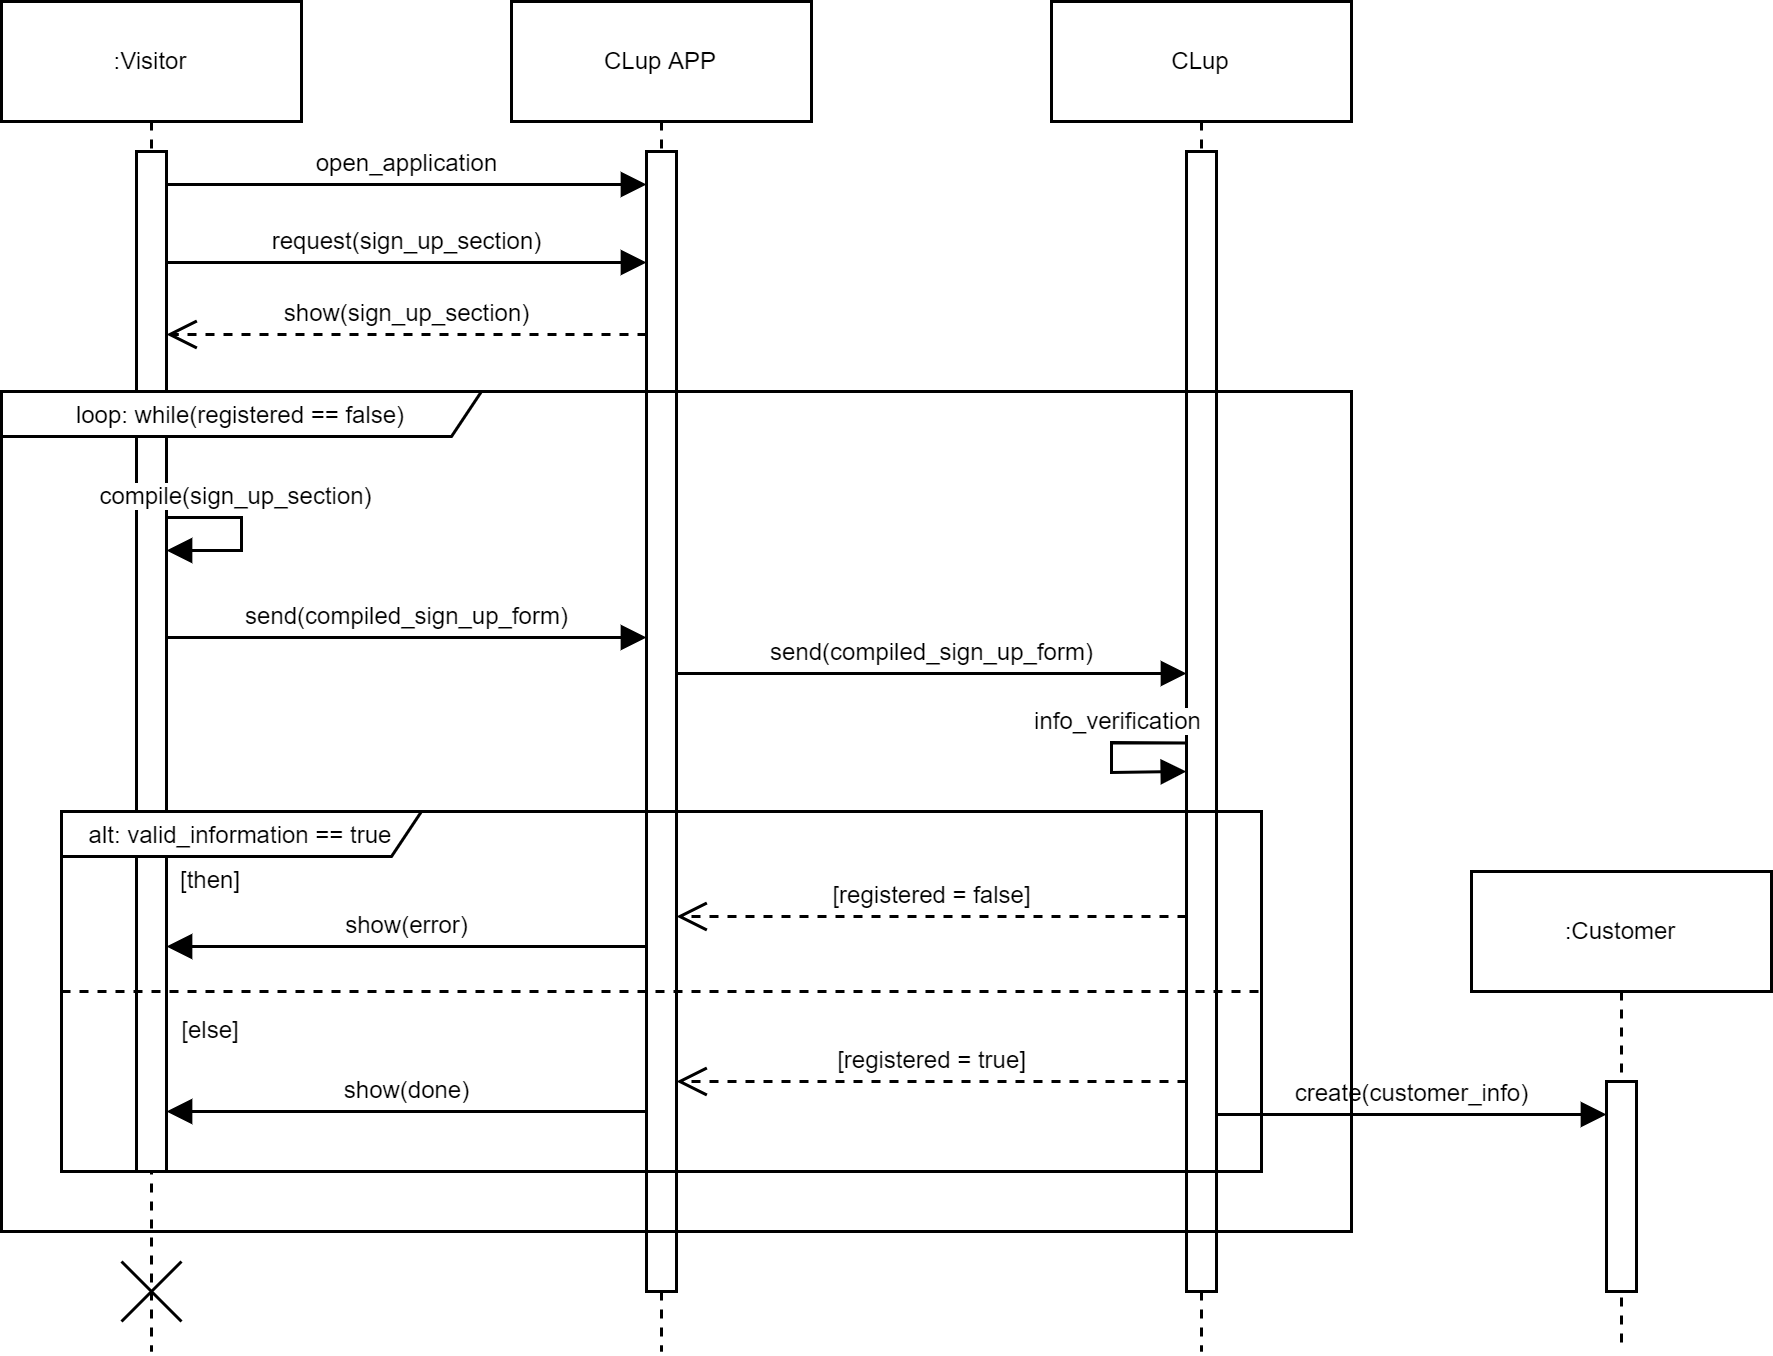
\includegraphics[width=\textwidth]{seq_diagr1.png}
    \caption{Registration to CLup as Customer}
\end{figure}

\begin{figure}
    \centering
    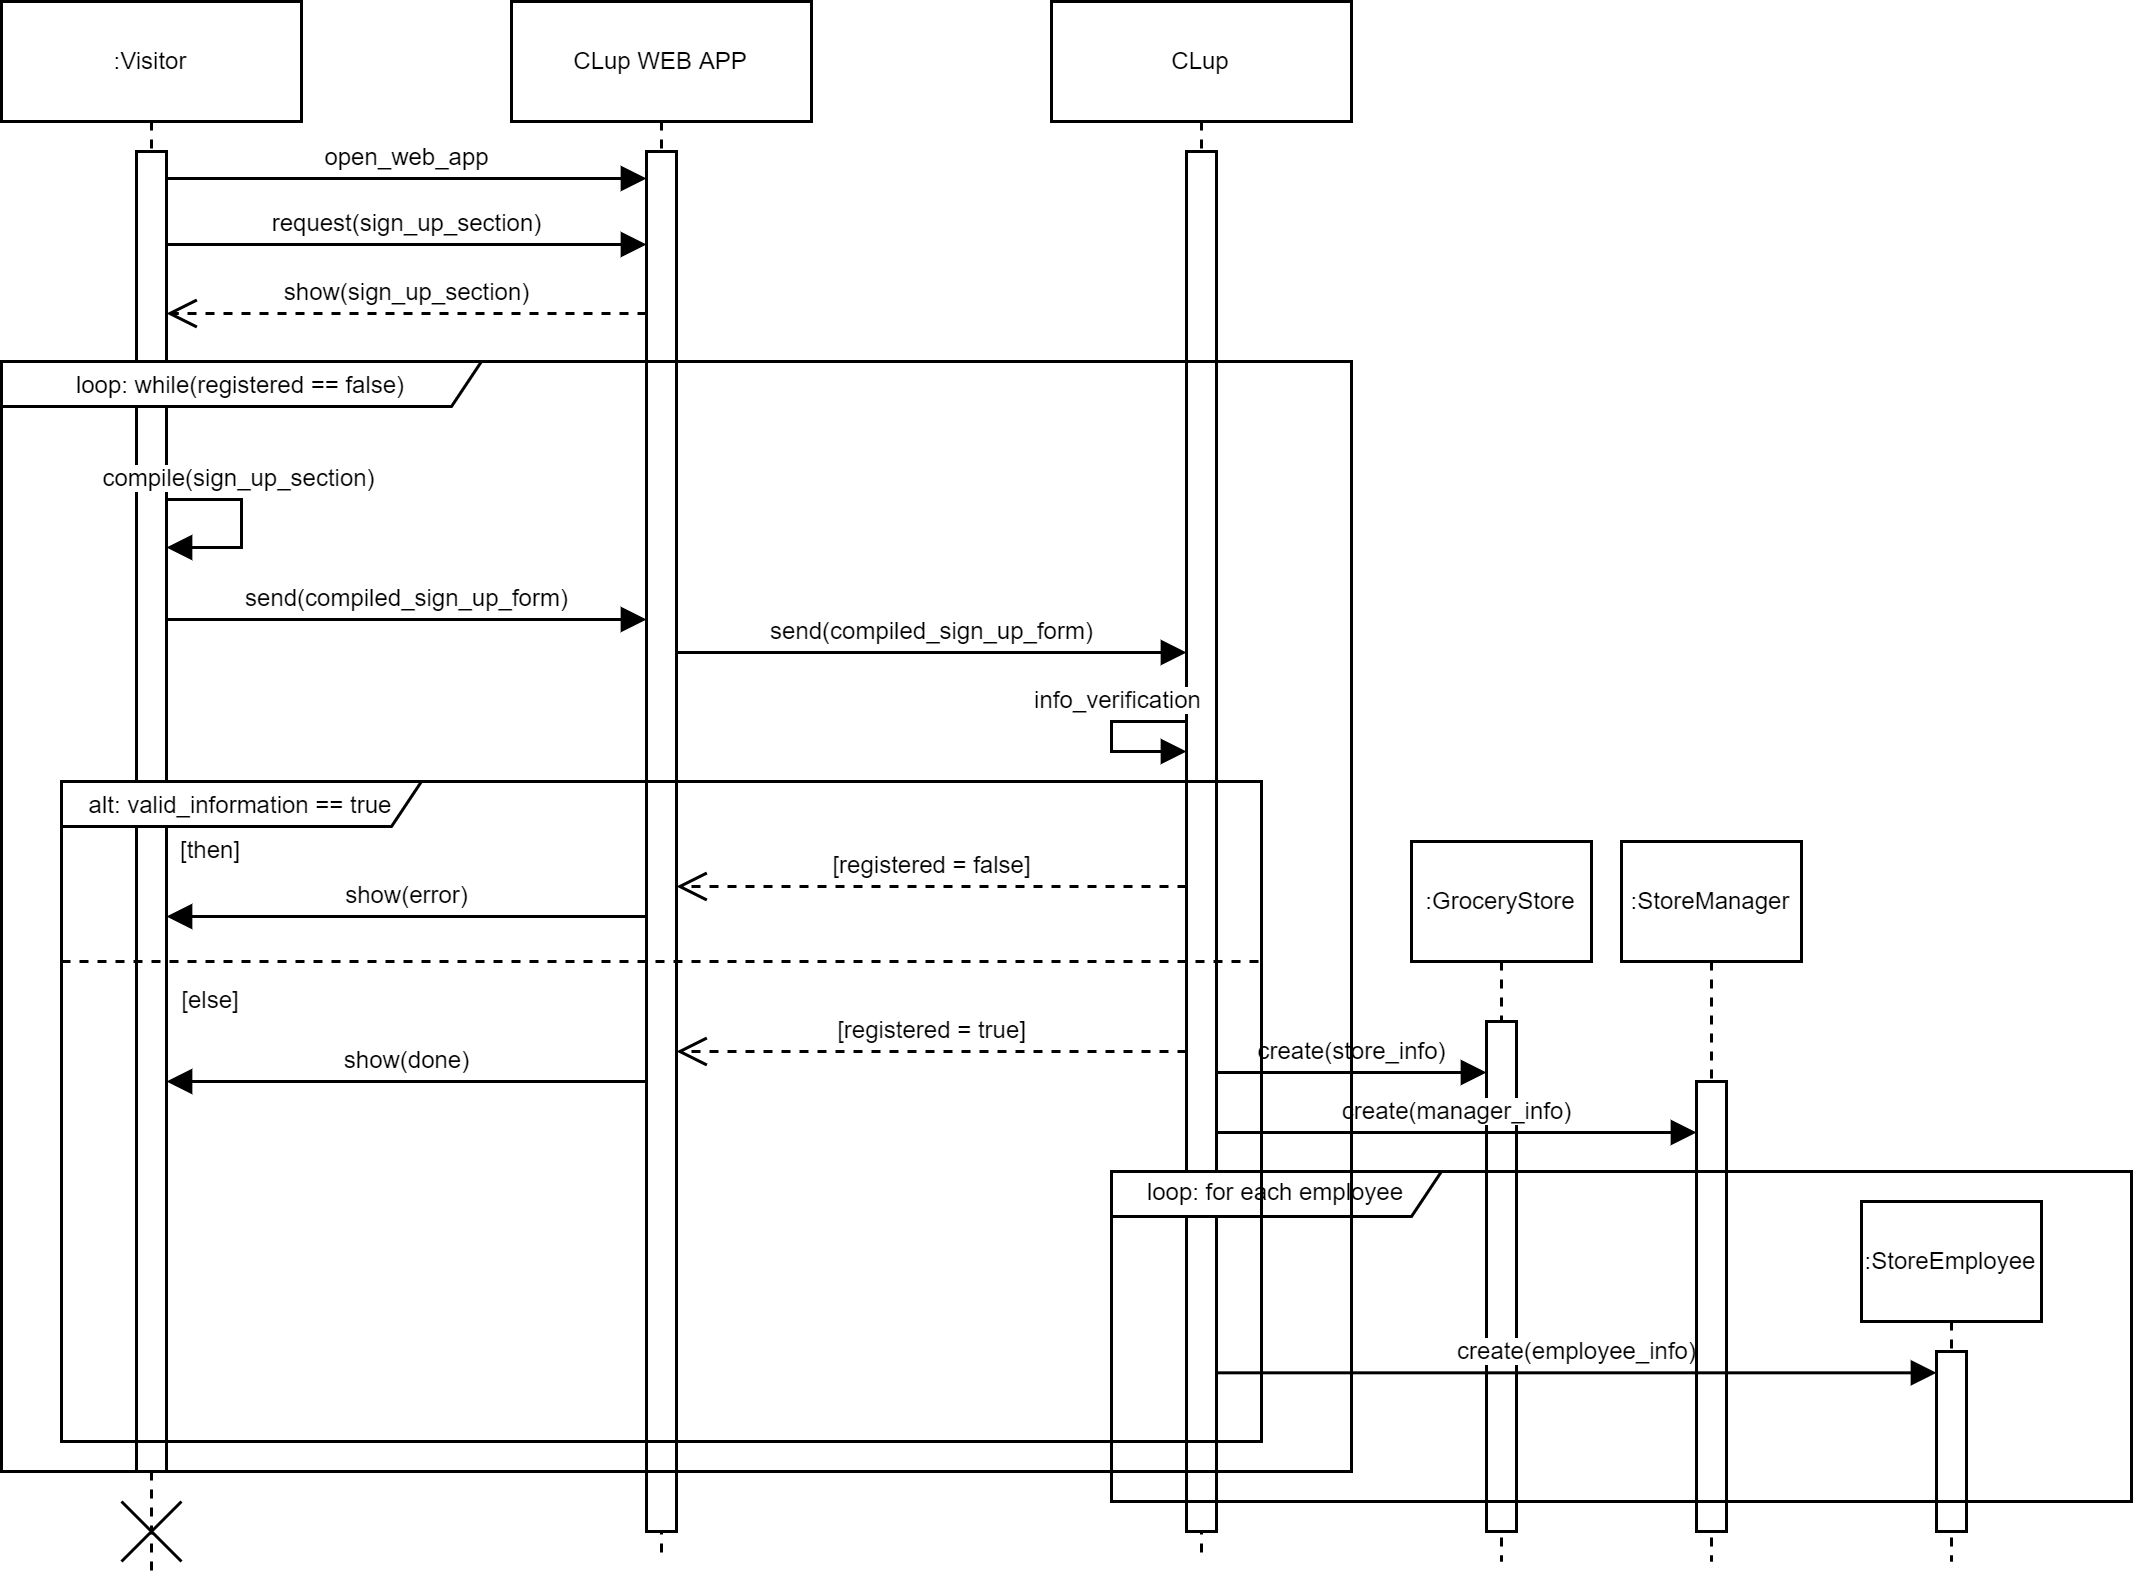
\includegraphics[width=\textwidth]{seq_diagr2.png}
    \caption{Registration to CLup as Store Manager}
\end{figure}

\begin{figure}
    \centering
    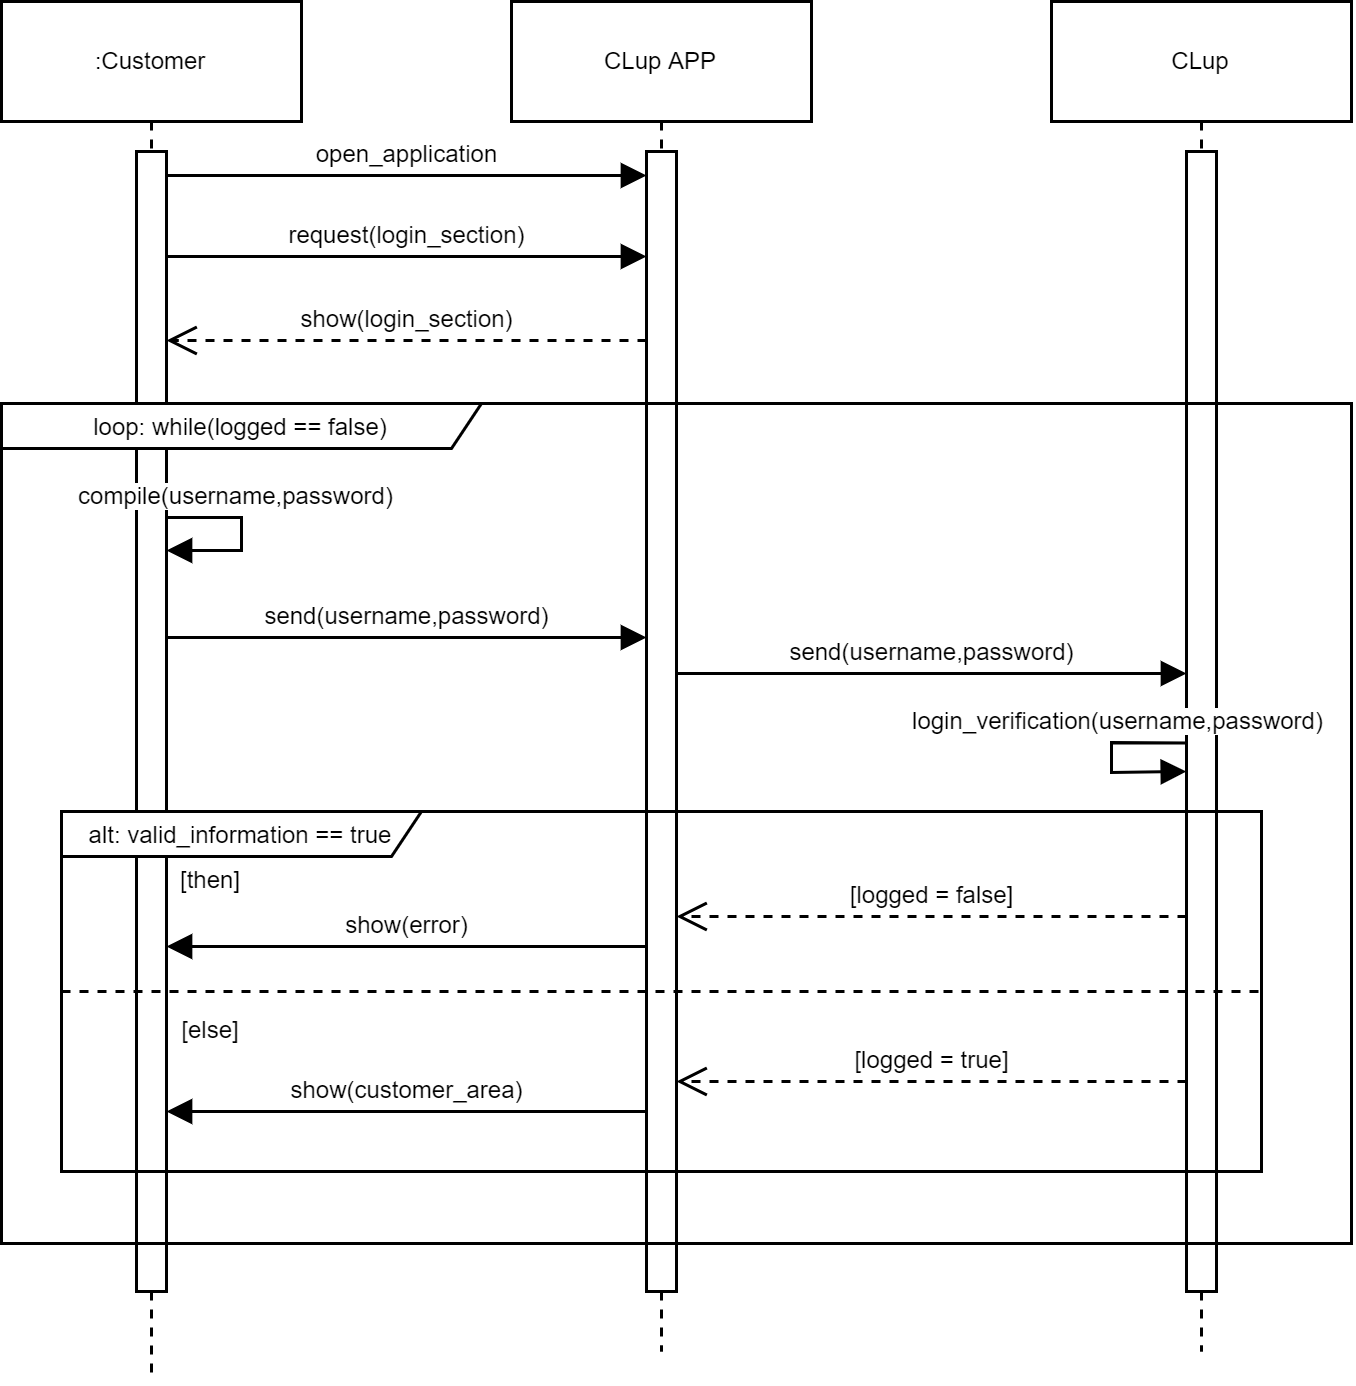
\includegraphics[width=\textwidth]{seq_diagr3.png}
    \caption{Login to the application}
\end{figure}

\begin{figure}
    \centering
    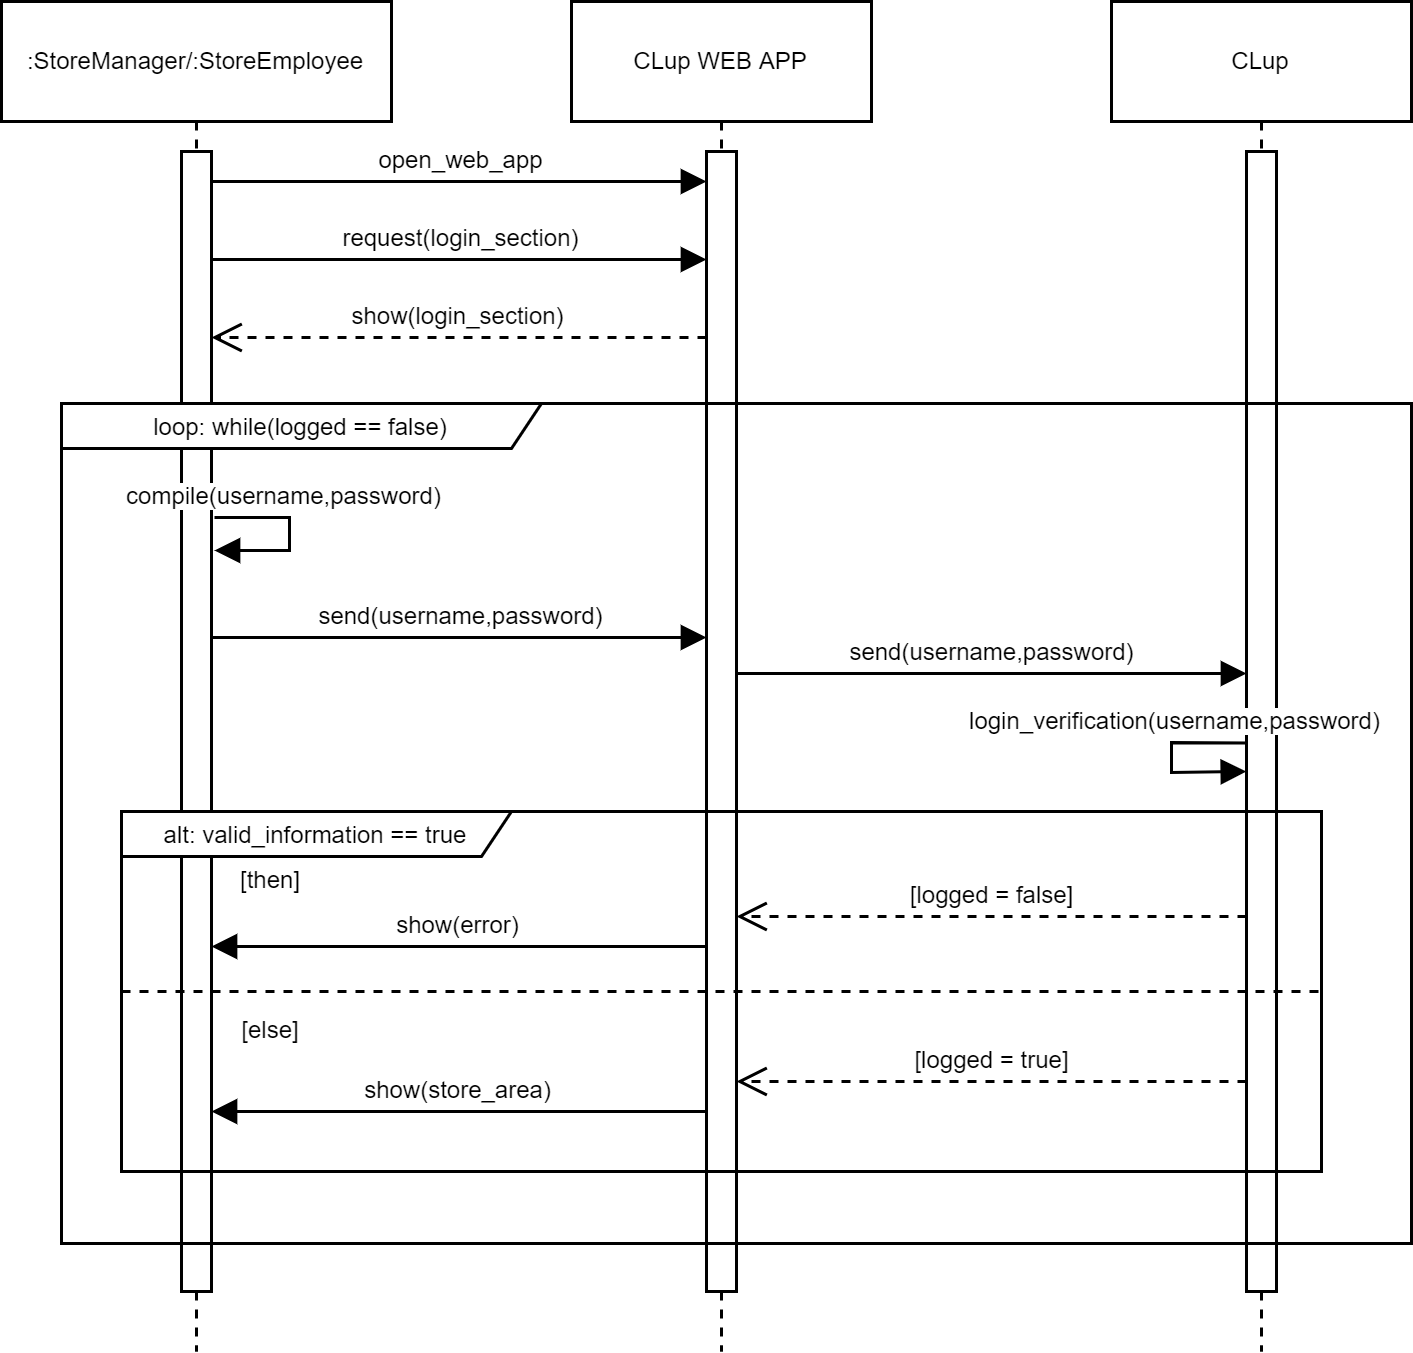
\includegraphics[width=\textwidth]{seq_diagr4.png}
    \caption{Login to the web app}
\end{figure}

\begin{figure}
    \centering
    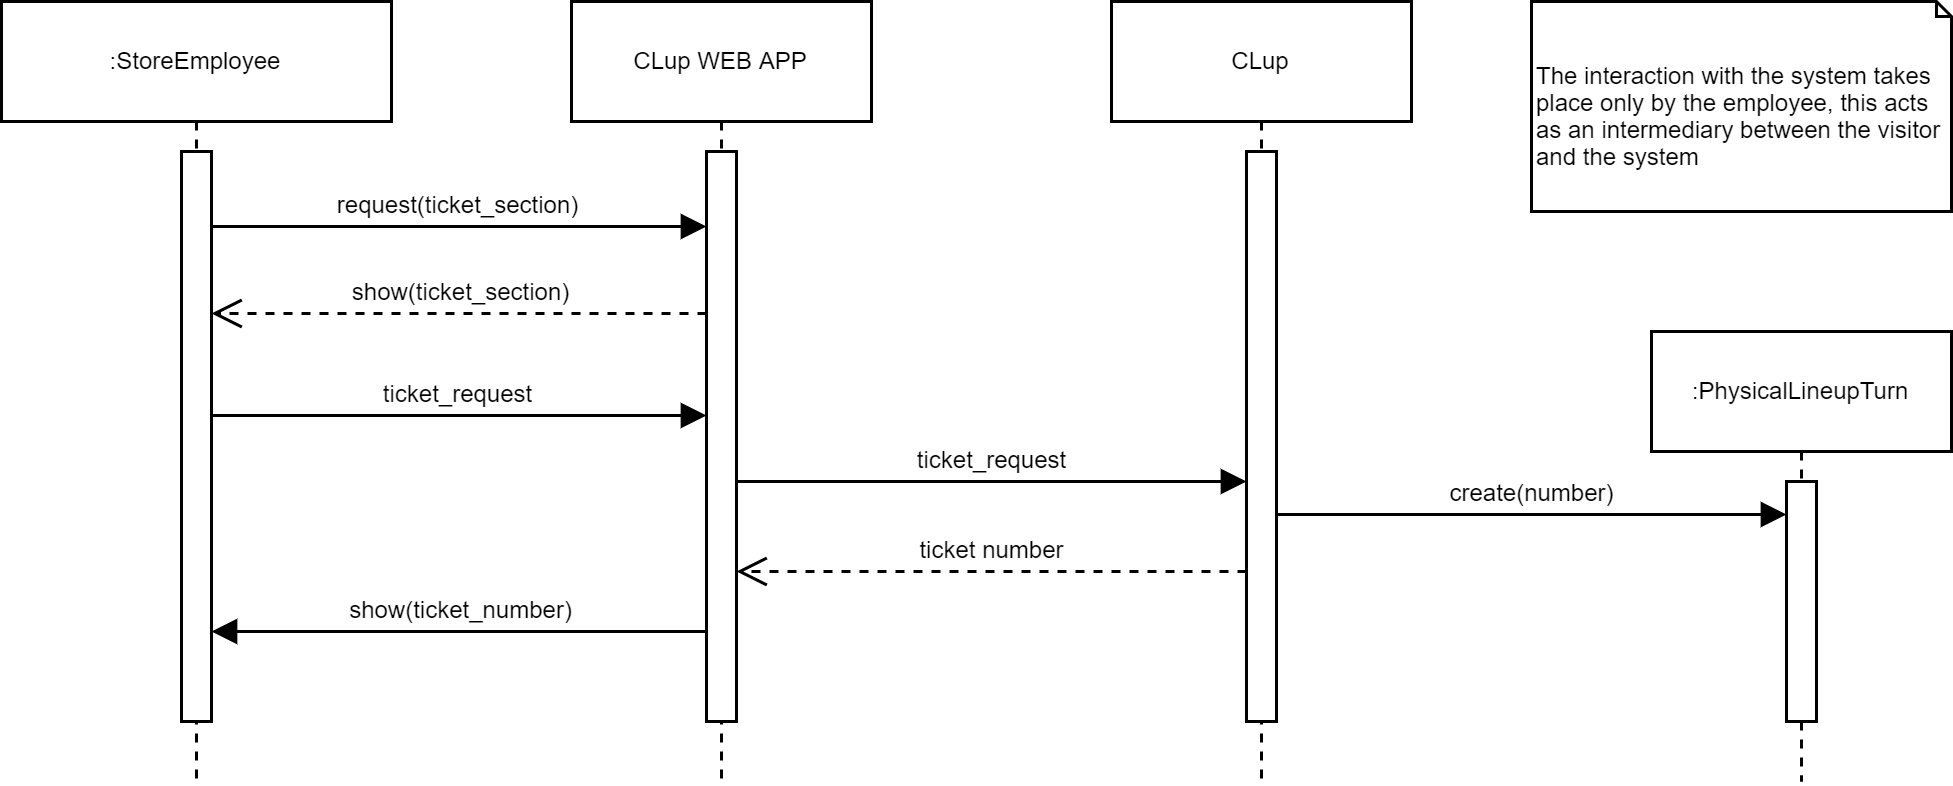
\includegraphics[width=\textwidth]{seq_diagr5.png}
    \caption{Lining up via store}
\end{figure}

\begin{figure}
    \centering
    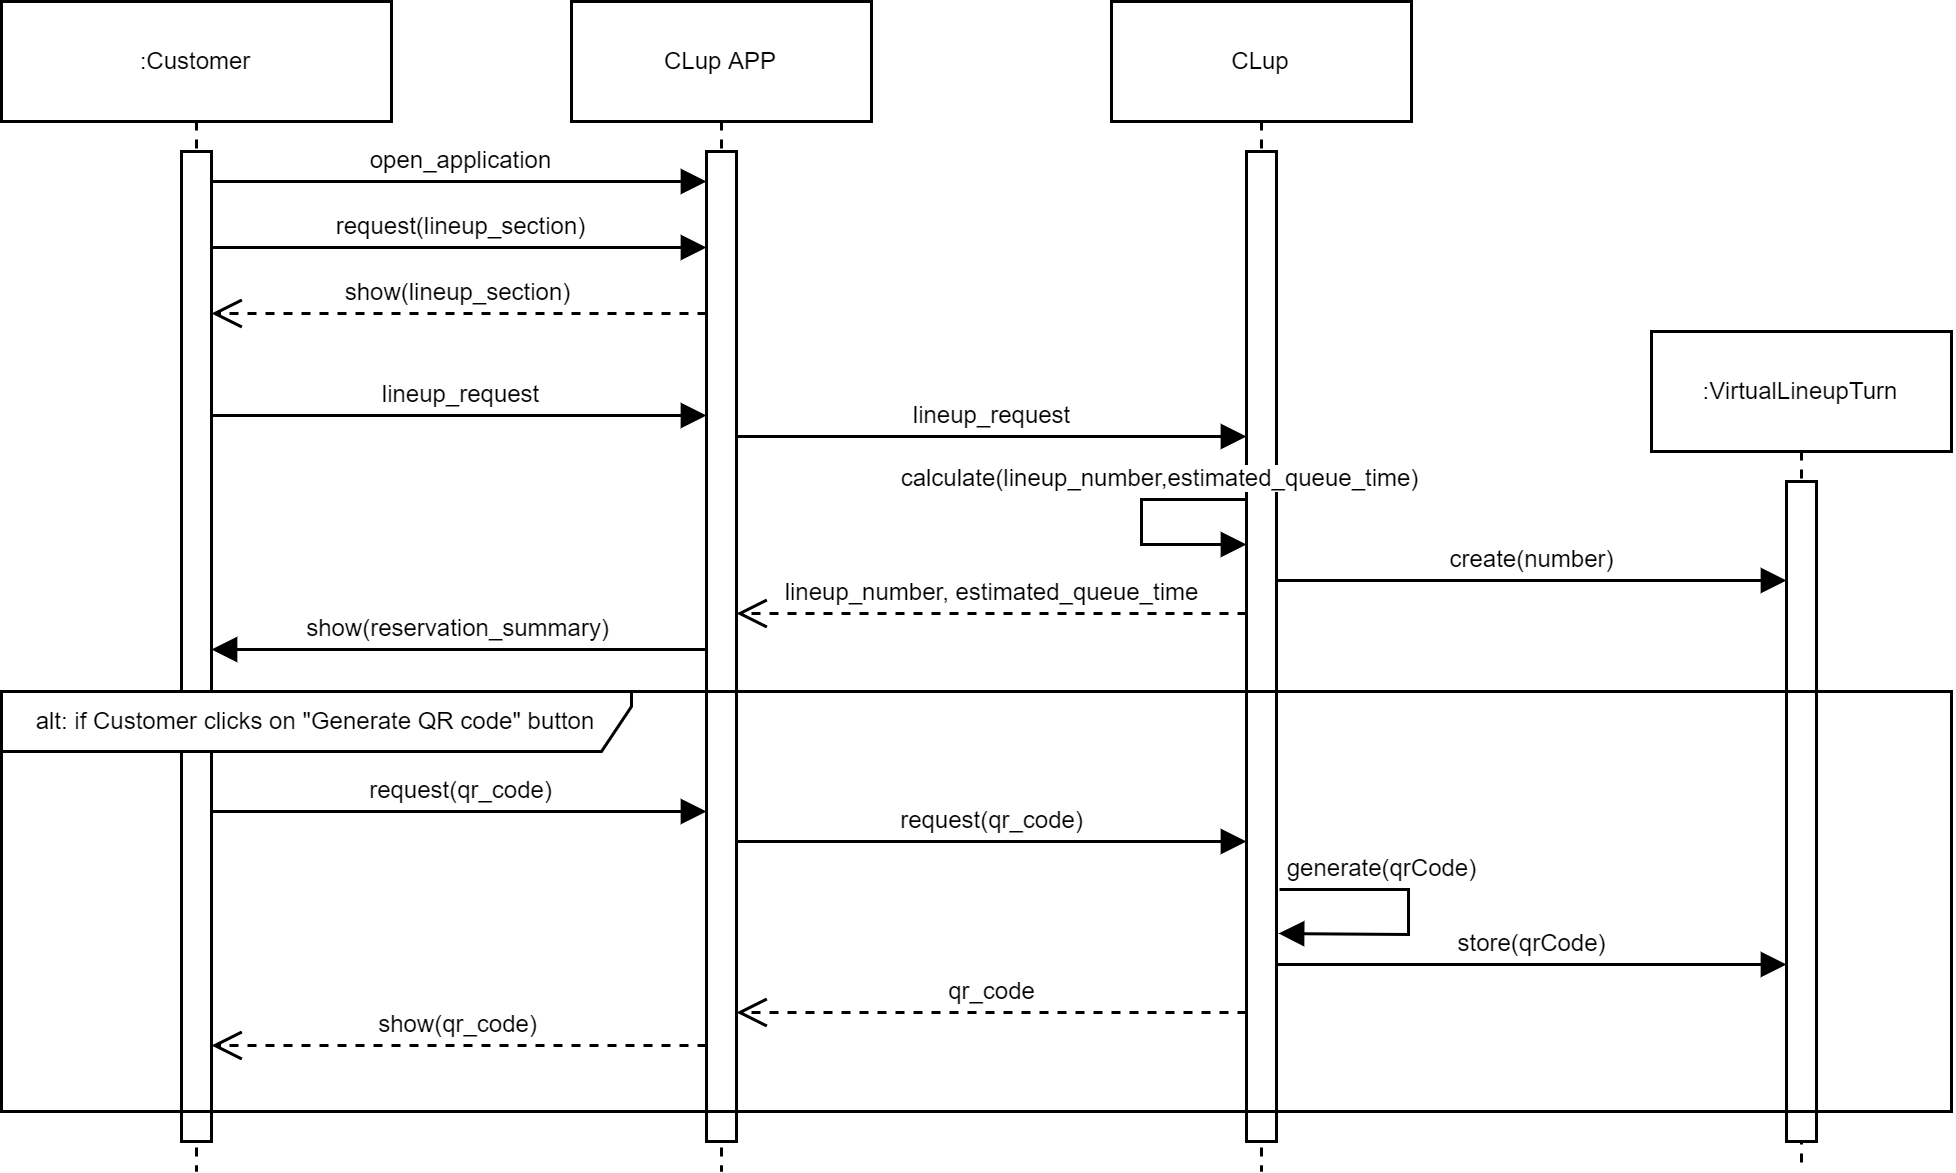
\includegraphics[width=\textwidth]{seq_diagr6.png}
    \caption{Lining up via app}
\end{figure}

\begin{figure}
    \centering
    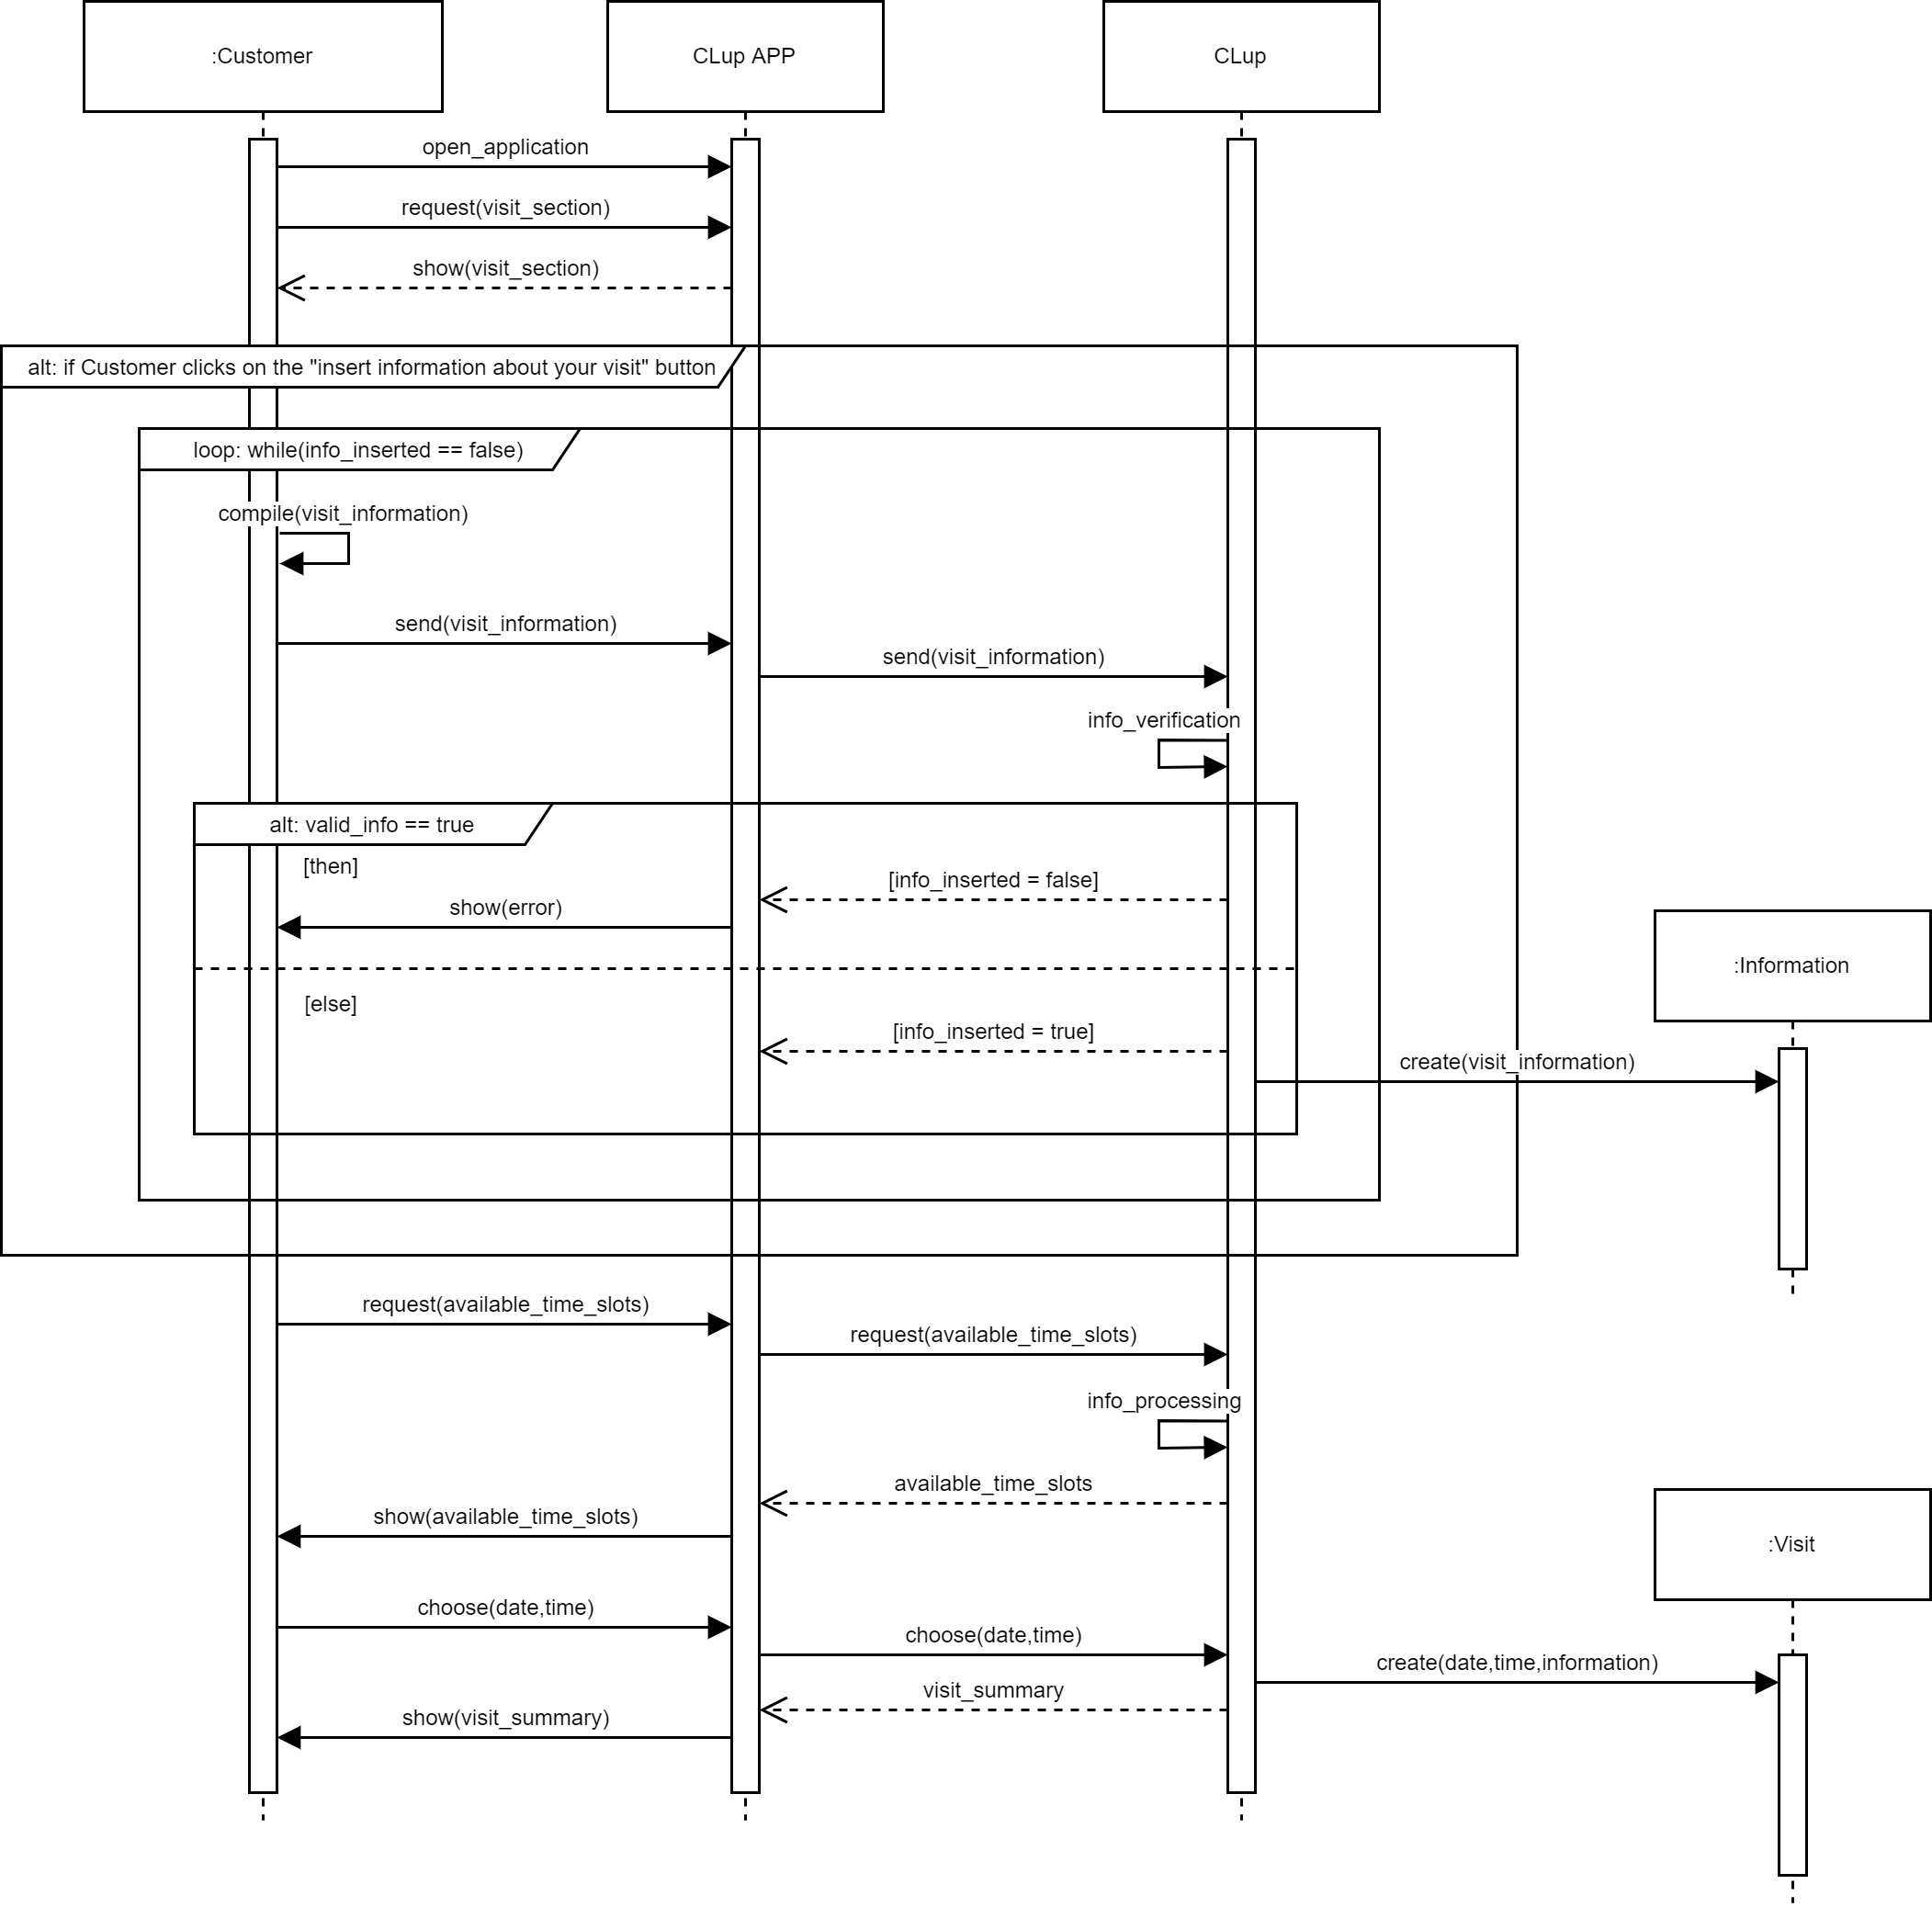
\includegraphics[width=\textwidth]{seq_diagr7.png}
    \caption{Book a visit}
\end{figure}

\begin{figure}
    \centering
    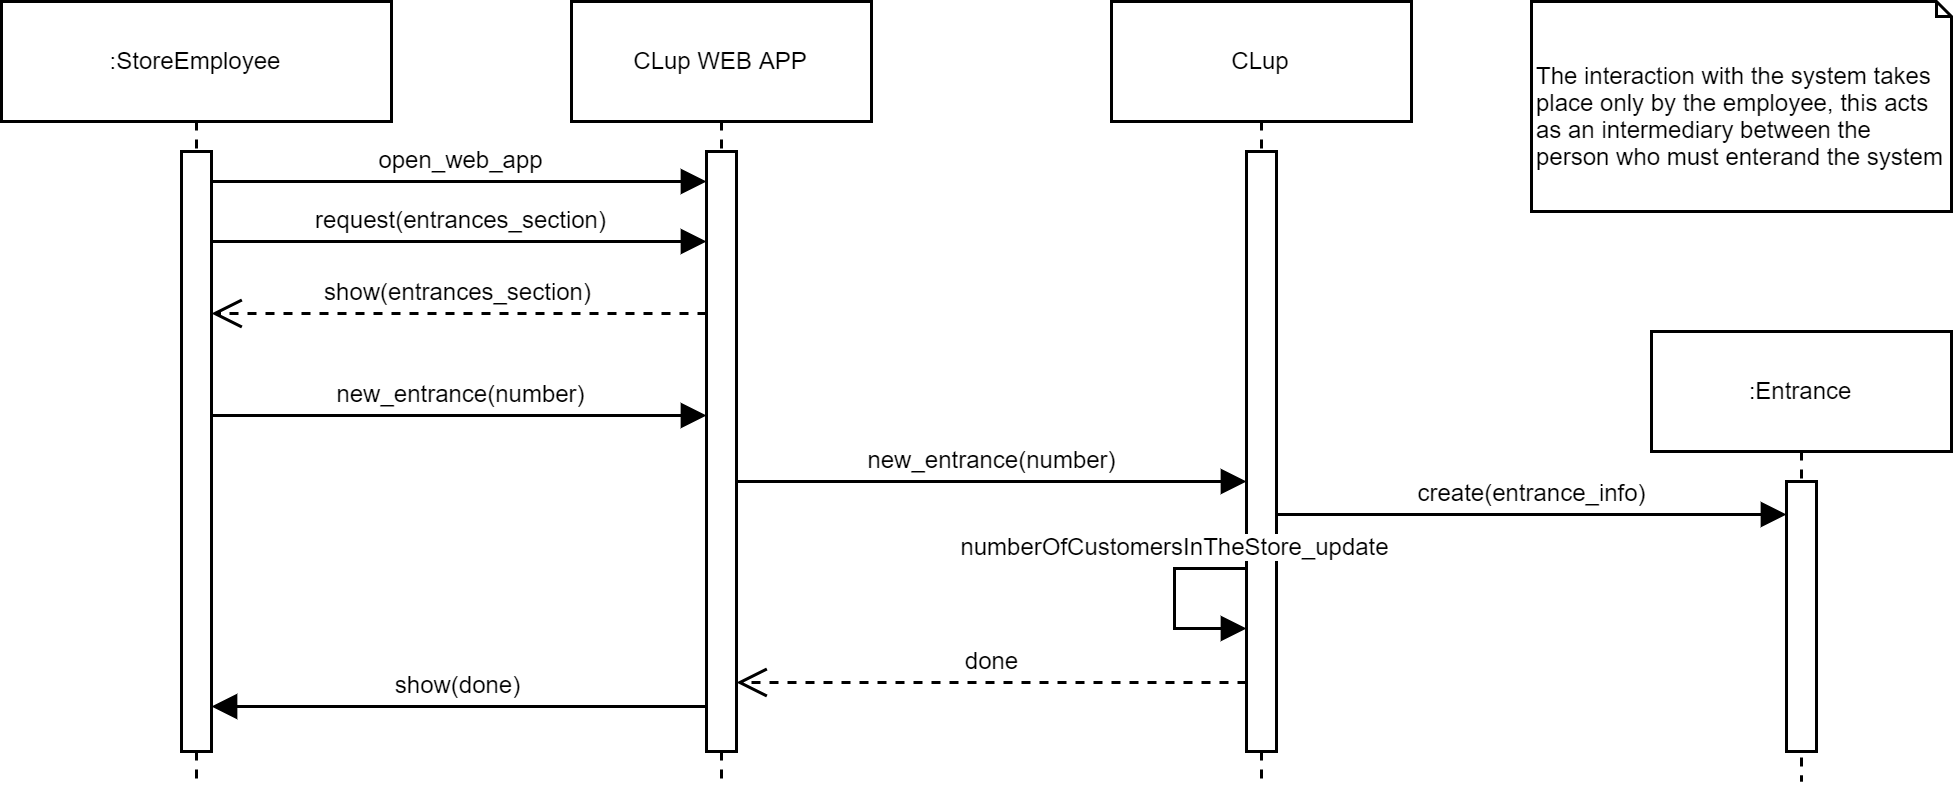
\includegraphics[width=\textwidth]{seq_diagr8.png}
    \caption{Enter the store without QR code after lineup reservation}
\end{figure}

\begin{figure}
    \centering
    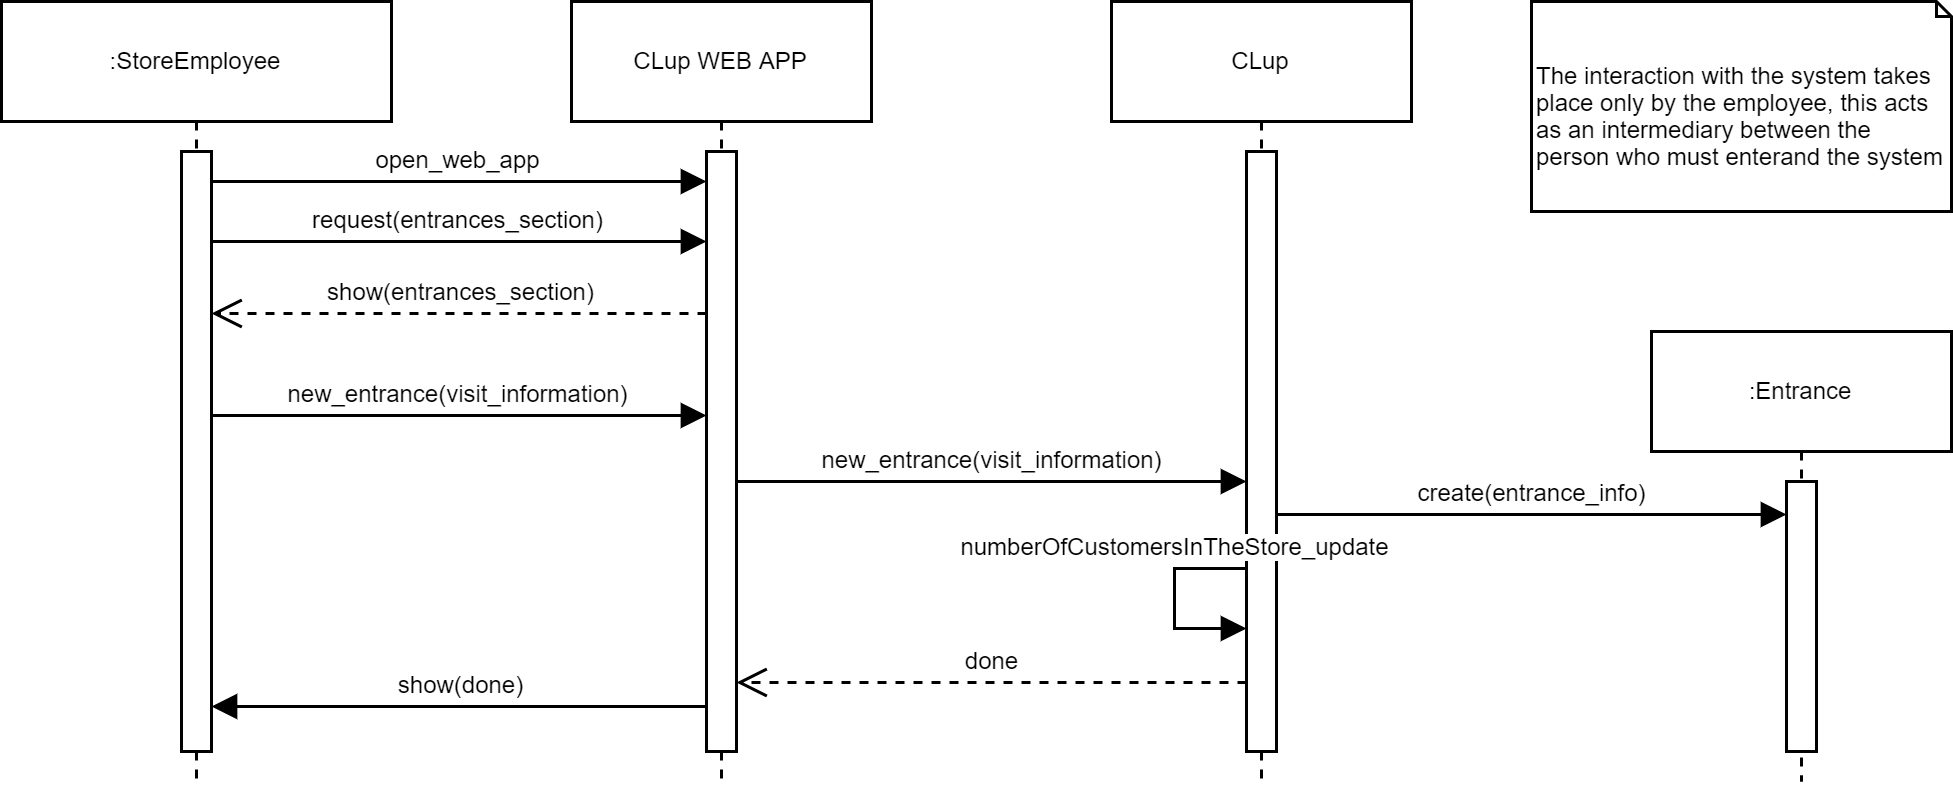
\includegraphics[width=\textwidth]{seq_diagr9.png}
    \caption{Enter the store without QR code for a visit}
\end{figure}

\begin{figure}
    \centering
    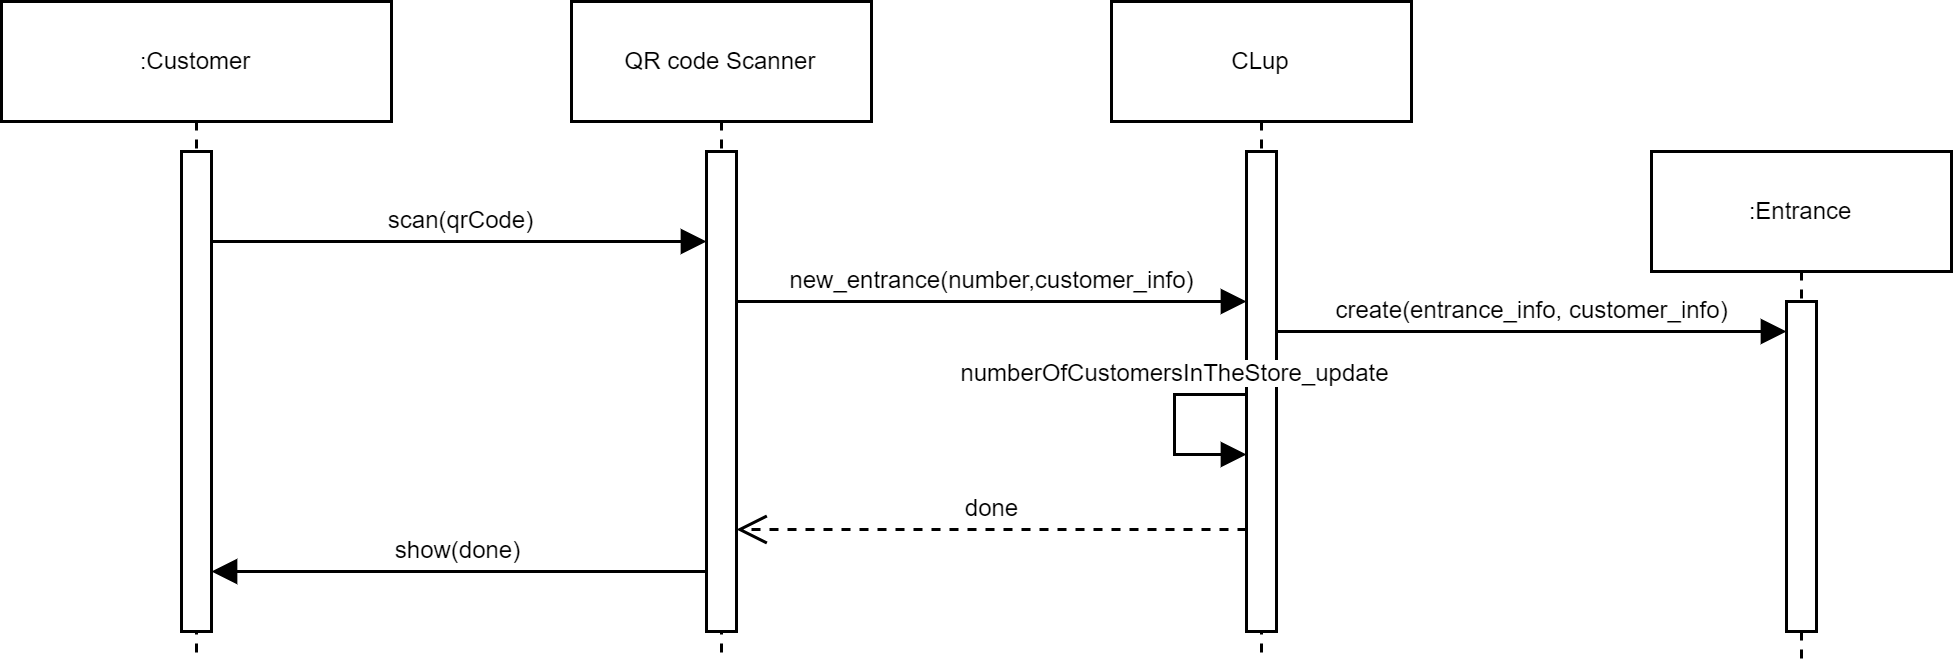
\includegraphics[width=\textwidth]{seq_diagr10.png}
    \caption{Enter the store with a QR code}
\end{figure}

\begin{figure}
    \centering
    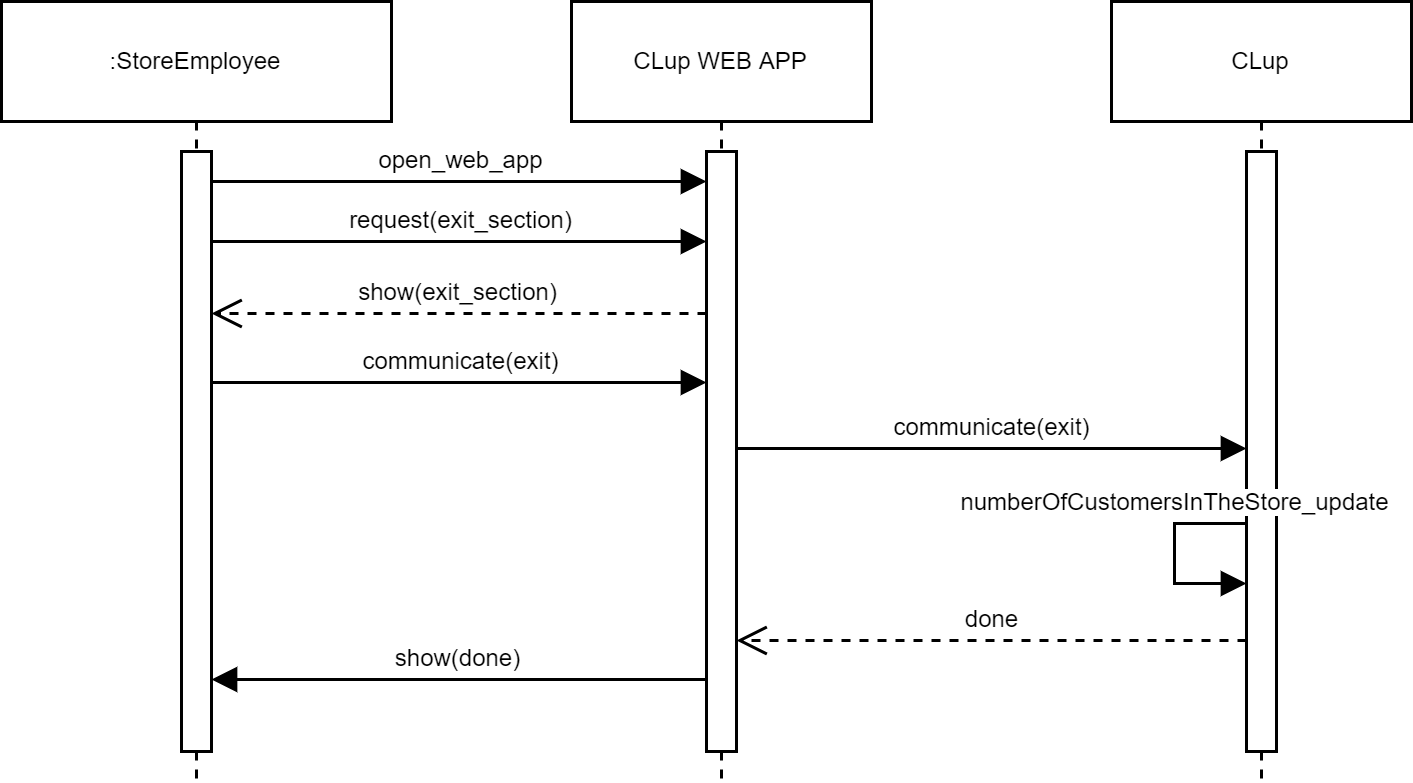
\includegraphics[width=\textwidth]{seq_diagr11.png}
    \caption{Register exit from store}
\end{figure}

\begin{figure}
    \centering
    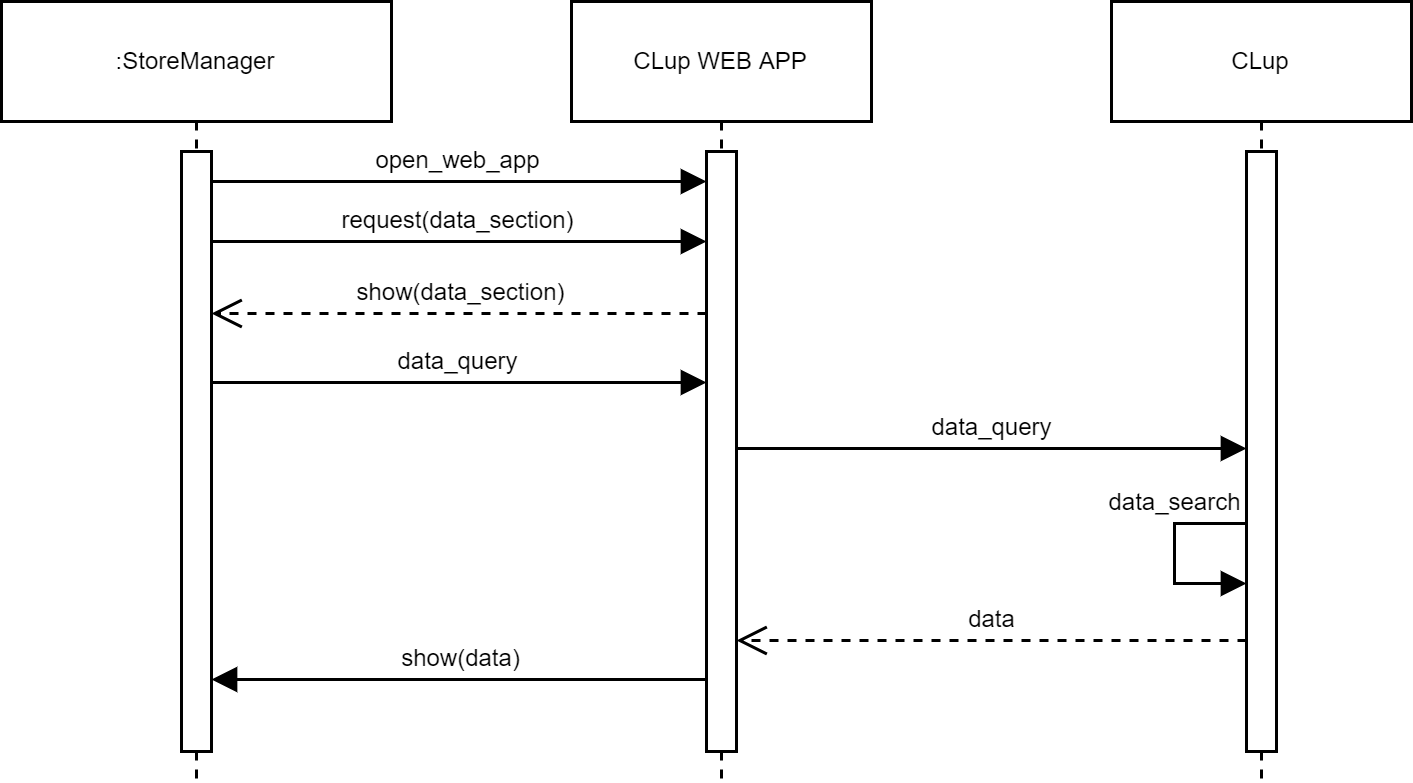
\includegraphics[width=\textwidth]{seq_diagr12.png}
    \caption{Display data of the accesses made through QR code}
\end{figure}

\clearpage